\documentclass[a4paper]{book}
\usepackage{a4wide}
\usepackage{makeidx}
\usepackage{graphicx}
\usepackage{multicol}
\usepackage{float}
\usepackage{listings}
\usepackage{color}
\usepackage{textcomp}
\usepackage{alltt}
\usepackage{times}
\usepackage{ifpdf}
\ifpdf
\usepackage[pdftex,
            pagebackref=true,
            colorlinks=true,
            linkcolor=blue,
            unicode
           ]{hyperref}
\else
\usepackage[ps2pdf,
            pagebackref=true,
            colorlinks=true,
            linkcolor=blue,
            unicode
           ]{hyperref}
\usepackage{pspicture}
\fi
\usepackage[utf8]{inputenc}
\usepackage{doxygen}
\lstset{language=C++,inputencoding=utf8,basicstyle=\footnotesize,breaklines=true,breakatwhitespace=true,tabsize=8,numbers=left }
\makeindex
\setcounter{tocdepth}{3}
\renewcommand{\footrulewidth}{0.4pt}
\begin{document}
\hypersetup{pageanchor=false}
\begin{titlepage}
\vspace*{7cm}
\begin{center}
{\Large WaCState }\\
\vspace*{1cm}
{\large Generated by Doxygen 1.6.3}\\
\vspace*{0.5cm}
{\small Wed Dec 15 16:43:23 2010}\\
\end{center}
\end{titlepage}
\clearemptydoublepage
\pagenumbering{roman}
\tableofcontents
\clearemptydoublepage
\pagenumbering{arabic}
\hypersetup{pageanchor=true}
\chapter{Namespace Index}
\section{Namespace List}
Here is a list of all namespaces with brief descriptions:\begin{DoxyCompactList}
\item\contentsline{section}{\hyperlink{namespacebr}{br} }{\pageref{namespacebr}}{}
\item\contentsline{section}{\hyperlink{namespacebr_1_1ufscar}{br::ufscar} }{\pageref{namespacebr_1_1ufscar}}{}
\item\contentsline{section}{\hyperlink{namespacebr_1_1ufscar_1_1lince}{br::ufscar::lince} }{\pageref{namespacebr_1_1ufscar_1_1lince}}{}
\item\contentsline{section}{\hyperlink{namespacebr_1_1ufscar_1_1lince_1_1ginga}{br::ufscar::lince::ginga} }{\pageref{namespacebr_1_1ufscar_1_1lince_1_1ginga}}{}
\item\contentsline{section}{\hyperlink{namespacebr_1_1ufscar_1_1lince_1_1ginga_1_1wac}{br::ufscar::lince::ginga::wac} }{\pageref{namespacebr_1_1ufscar_1_1lince_1_1ginga_1_1wac}}{}
\item\contentsline{section}{\hyperlink{namespacebr_1_1ufscar_1_1lince_1_1ginga_1_1wac_1_1state}{br::ufscar::lince::ginga::wac::state} }{\pageref{namespacebr_1_1ufscar_1_1lince_1_1ginga_1_1wac_1_1state}}{}
\end{DoxyCompactList}

\chapter{Data Structure Index}
\section{Class Hierarchy}
This inheritance list is sorted roughly, but not completely, alphabetically:\begin{DoxyCompactList}
\item \contentsline{section}{br::ufscar::lince::ginga::wac::state::IContextProvider}{\pageref{classbr_1_1ufscar_1_1lince_1_1ginga_1_1wac_1_1state_1_1IContextProvider}}{}
\item \contentsline{section}{br::ufscar::lince::ginga::wac::state::IElementaryState}{\pageref{classbr_1_1ufscar_1_1lince_1_1ginga_1_1wac_1_1state_1_1IElementaryState}}{}
\begin{DoxyCompactList}
\item \contentsline{section}{br::ufscar::lince::ginga::wac::state::ElementaryState}{\pageref{classbr_1_1ufscar_1_1lince_1_1ginga_1_1wac_1_1state_1_1ElementaryState}}{}
\end{DoxyCompactList}
\item \contentsline{section}{br::ufscar::lince::ginga::wac::state::IPresentationState}{\pageref{classbr_1_1ufscar_1_1lince_1_1ginga_1_1wac_1_1state_1_1IPresentationState}}{}
\begin{DoxyCompactList}
\item \contentsline{section}{br::ufscar::lince::ginga::wac::state::PresentationState}{\pageref{classbr_1_1ufscar_1_1lince_1_1ginga_1_1wac_1_1state_1_1PresentationState}}{}
\end{DoxyCompactList}
\item \contentsline{section}{br::ufscar::lince::ginga::wac::state::IStateManager}{\pageref{classbr_1_1ufscar_1_1lince_1_1ginga_1_1wac_1_1state_1_1IStateManager}}{}
\begin{DoxyCompactList}
\item \contentsline{section}{br::ufscar::lince::ginga::wac::state::StateManager}{\pageref{classbr_1_1ufscar_1_1lince_1_1ginga_1_1wac_1_1state_1_1StateManager}}{}
\end{DoxyCompactList}
\item \contentsline{section}{br::ufscar::lince::ginga::wac::state::IStateProvider}{\pageref{classbr_1_1ufscar_1_1lince_1_1ginga_1_1wac_1_1state_1_1IStateProvider}}{}
\end{DoxyCompactList}

\chapter{Data Structure Index}
\section{Data Structures}
Here are the data structures with brief descriptions:\begin{DoxyCompactList}
\item\contentsline{section}{\hyperlink{classbr_1_1ufscar_1_1lince_1_1ginga_1_1wac_1_1editing_1_1ClientEditingManager}{br::ufscar::lince::ginga::wac::editing::ClientEditingManager} (Permite a aplicações desenvolvidas pelo usuário realizar anotações e edições ao vivo em um documento NCL Esta classe basicamente facilita a criação de aplicações de anotação e edição ao vivo do lado cliente, pois faz parte das tarefas necessárias para aplicações deste tipo, além de permitir retroceder de alterações erroneas e fazer um log das alterações )}{\pageref{classbr_1_1ufscar_1_1lince_1_1ginga_1_1wac_1_1editing_1_1ClientEditingManager}}{}
\item\contentsline{section}{\hyperlink{classbr_1_1ufscar_1_1lince_1_1ginga_1_1wac_1_1editing_1_1EditingCommand}{br::ufscar::lince::ginga::wac::editing::EditingCommand} (Classe que encapsula comandos de edição ao vivo do usuário )}{\pageref{classbr_1_1ufscar_1_1lince_1_1ginga_1_1wac_1_1editing_1_1EditingCommand}}{}
\item\contentsline{section}{\hyperlink{classbr_1_1ufscar_1_1lince_1_1ginga_1_1wac_1_1editing_1_1IClientEditing}{br::ufscar::lince::ginga::wac::editing::IClientEditing} (Interface utilizada pelas aplicações do cliente para utilizar os serviçõs do módulo ClientEditig )}{\pageref{classbr_1_1ufscar_1_1lince_1_1ginga_1_1wac_1_1editing_1_1IClientEditing}}{}
\item\contentsline{section}{\hyperlink{classbr_1_1ufscar_1_1lince_1_1ginga_1_1wac_1_1editing_1_1IFormatterAdapter}{br::ufscar::lince::ginga::wac::editing::IFormatterAdapter} (Interface que permite que as classes do módulo Wac-\/Editing enviem mensagem a classe Formatter do módulo Formatter )}{\pageref{classbr_1_1ufscar_1_1lince_1_1ginga_1_1wac_1_1editing_1_1IFormatterAdapter}}{}
\item\contentsline{section}{\hyperlink{classbr_1_1ufscar_1_1lince_1_1ginga_1_1wac_1_1editing_1_1ILinkAction}{br::ufscar::lince::ginga::wac::editing::ILinkAction} (Interface pela qual é possivel obter informações sobre os links do módulo Formatter )}{\pageref{classbr_1_1ufscar_1_1lince_1_1ginga_1_1wac_1_1editing_1_1ILinkAction}}{}
\item\contentsline{section}{\hyperlink{classbr_1_1ufscar_1_1lince_1_1ginga_1_1wac_1_1editing_1_1IMode}{br::ufscar::lince::ginga::wac::editing::IMode} (Interface que permite a manipulação dos modos de exibição )}{\pageref{classbr_1_1ufscar_1_1lince_1_1ginga_1_1wac_1_1editing_1_1IMode}}{}
\item\contentsline{section}{\hyperlink{classbr_1_1ufscar_1_1lince_1_1ginga_1_1wac_1_1editing_1_1IObjectMode}{br::ufscar::lince::ginga::wac::editing::IObjectMode} (Interface que permite ao módulo Wac-\/Editing Manipular ExecutionObjetcs do módulo Formatter )}{\pageref{classbr_1_1ufscar_1_1lince_1_1ginga_1_1wac_1_1editing_1_1IObjectMode}}{}
\item\contentsline{section}{\hyperlink{classbr_1_1ufscar_1_1lince_1_1ginga_1_1wac_1_1editing_1_1ISchedulerAdapter}{br::ufscar::lince::ginga::wac::editing::ISchedulerAdapter} (Interface pela qual este módulo envia mensagem a classe Scheduler do módulo Formatter )}{\pageref{classbr_1_1ufscar_1_1lince_1_1ginga_1_1wac_1_1editing_1_1ISchedulerAdapter}}{}
\item\contentsline{section}{\hyperlink{classbr_1_1ufscar_1_1lince_1_1ginga_1_1wac_1_1editing_1_1ModeManager}{br::ufscar::lince::ginga::wac::editing::ModeManager} (Classe responsável manipular os modos de exibição do cliente e da emissora )}{\pageref{classbr_1_1ufscar_1_1lince_1_1ginga_1_1wac_1_1editing_1_1ModeManager}}{}
\end{DoxyCompactList}

\chapter{File Index}
\section{File List}
Here is a list of all files with brief descriptions:\begin{DoxyCompactList}
\item\contentsline{section}{include/\hyperlink{INclGenerator_8h}{INclGenerator.h} }{\pageref{INclGenerator_8h}}{}
\item\contentsline{section}{include/\hyperlink{NclFileGenerator_8h}{NclFileGenerator.h} }{\pageref{NclFileGenerator_8h}}{}
\item\contentsline{section}{include/\hyperlink{NclGenerator_8h}{NclGenerator.h} }{\pageref{NclGenerator_8h}}{}
\item\contentsline{section}{include/\hyperlink{UnsupportedNclEntityException_8h}{UnsupportedNclEntityException.h} }{\pageref{UnsupportedNclEntityException_8h}}{}
\item\contentsline{section}{include/generables/\hyperlink{AnchorGenerator_8h}{AnchorGenerator.h} }{\pageref{AnchorGenerator_8h}}{}
\item\contentsline{section}{include/generables/\hyperlink{AssessmentStatementGenerator_8h}{AssessmentStatementGenerator.h} }{\pageref{AssessmentStatementGenerator_8h}}{}
\item\contentsline{section}{include/generables/\hyperlink{AttributeAssessmentGenerator_8h}{AttributeAssessmentGenerator.h} }{\pageref{AttributeAssessmentGenerator_8h}}{}
\item\contentsline{section}{include/generables/\hyperlink{BindGenerator_8h}{BindGenerator.h} }{\pageref{BindGenerator_8h}}{}
\item\contentsline{section}{include/generables/\hyperlink{CausalConnectorGenerator_8h}{CausalConnectorGenerator.h} }{\pageref{CausalConnectorGenerator_8h}}{}
\item\contentsline{section}{include/generables/\hyperlink{CausalLinkGenerator_8h}{CausalLinkGenerator.h} }{\pageref{CausalLinkGenerator_8h}}{}
\item\contentsline{section}{include/generables/\hyperlink{CircleSpatialAnchorGenerator_8h}{CircleSpatialAnchorGenerator.h} }{\pageref{CircleSpatialAnchorGenerator_8h}}{}
\item\contentsline{section}{include/generables/\hyperlink{CompositeRuleGenerator_8h}{CompositeRuleGenerator.h} }{\pageref{CompositeRuleGenerator_8h}}{}
\item\contentsline{section}{include/generables/\hyperlink{CompoundActionGenerator_8h}{CompoundActionGenerator.h} }{\pageref{CompoundActionGenerator_8h}}{}
\item\contentsline{section}{include/generables/\hyperlink{CompoundConditionGenerator_8h}{CompoundConditionGenerator.h} }{\pageref{CompoundConditionGenerator_8h}}{}
\item\contentsline{section}{include/generables/\hyperlink{CompoundStatementGenerator_8h}{CompoundStatementGenerator.h} }{\pageref{CompoundStatementGenerator_8h}}{}
\item\contentsline{section}{include/generables/\hyperlink{ConnectorBaseGenerator_8h}{ConnectorBaseGenerator.h} }{\pageref{ConnectorBaseGenerator_8h}}{}
\item\contentsline{section}{include/generables/\hyperlink{ContentNodeGenerator_8h}{ContentNodeGenerator.h} }{\pageref{ContentNodeGenerator_8h}}{}
\item\contentsline{section}{include/generables/\hyperlink{ContextNodeGenerator_8h}{ContextNodeGenerator.h} }{\pageref{ContextNodeGenerator_8h}}{}
\item\contentsline{section}{include/generables/\hyperlink{DescriptorBaseGenerator_8h}{DescriptorBaseGenerator.h} }{\pageref{DescriptorBaseGenerator_8h}}{}
\item\contentsline{section}{include/generables/\hyperlink{DescriptorGenerator_8h}{DescriptorGenerator.h} }{\pageref{DescriptorGenerator_8h}}{}
\item\contentsline{section}{include/generables/\hyperlink{DescriptorSwitchGenerator_8h}{DescriptorSwitchGenerator.h} }{\pageref{DescriptorSwitchGenerator_8h}}{}
\item\contentsline{section}{include/generables/\hyperlink{Generable_8h}{Generable.h} }{\pageref{Generable_8h}}{}
\item\contentsline{section}{include/generables/\hyperlink{GeneratorUtil_8h}{GeneratorUtil.h} }{\pageref{GeneratorUtil_8h}}{}
\item\contentsline{section}{include/generables/\hyperlink{IntervalAnchorGenerator_8h}{IntervalAnchorGenerator.h} }{\pageref{IntervalAnchorGenerator_8h}}{}
\item\contentsline{section}{include/generables/\hyperlink{LabeledAnchorGenerator_8h}{LabeledAnchorGenerator.h} }{\pageref{LabeledAnchorGenerator_8h}}{}
\item\contentsline{section}{include/generables/\hyperlink{LayoutRegionGenerator_8h}{LayoutRegionGenerator.h} }{\pageref{LayoutRegionGenerator_8h}}{}
\item\contentsline{section}{include/generables/\hyperlink{NclDocumentGenerator_8h}{NclDocumentGenerator.h} }{\pageref{NclDocumentGenerator_8h}}{}
\item\contentsline{section}{include/generables/\hyperlink{ParameterGenerator_8h}{ParameterGenerator.h} }{\pageref{ParameterGenerator_8h}}{}
\item\contentsline{section}{include/generables/\hyperlink{PortGenerator_8h}{PortGenerator.h} }{\pageref{PortGenerator_8h}}{}
\item\contentsline{section}{include/generables/\hyperlink{PropertyAnchorGenerator_8h}{PropertyAnchorGenerator.h} }{\pageref{PropertyAnchorGenerator_8h}}{}
\item\contentsline{section}{include/generables/\hyperlink{RectangleSpatialAnchorGenerator_8h}{RectangleSpatialAnchorGenerator.h} }{\pageref{RectangleSpatialAnchorGenerator_8h}}{}
\item\contentsline{section}{include/generables/\hyperlink{RegionBaseGenerator_8h}{RegionBaseGenerator.h} }{\pageref{RegionBaseGenerator_8h}}{}
\item\contentsline{section}{include/generables/\hyperlink{RuleBaseGenerator_8h}{RuleBaseGenerator.h} }{\pageref{RuleBaseGenerator_8h}}{}
\item\contentsline{section}{include/generables/\hyperlink{SimpleActionGenerator_8h}{SimpleActionGenerator.h} }{\pageref{SimpleActionGenerator_8h}}{}
\item\contentsline{section}{include/generables/\hyperlink{SimpleConditionGenerator_8h}{SimpleConditionGenerator.h} }{\pageref{SimpleConditionGenerator_8h}}{}
\item\contentsline{section}{include/generables/\hyperlink{SimpleRuleGenerator_8h}{SimpleRuleGenerator.h} }{\pageref{SimpleRuleGenerator_8h}}{}
\item\contentsline{section}{include/generables/\hyperlink{SwitchNodeGenerator_8h}{SwitchNodeGenerator.h} }{\pageref{SwitchNodeGenerator_8h}}{}
\item\contentsline{section}{include/generables/\hyperlink{SwitchPortGenerator_8h}{SwitchPortGenerator.h} }{\pageref{SwitchPortGenerator_8h}}{}
\item\contentsline{section}{include/generables/\hyperlink{TextAnchorGenerator_8h}{TextAnchorGenerator.h} }{\pageref{TextAnchorGenerator_8h}}{}
\item\contentsline{section}{include/generables/\hyperlink{TransitionBaseGenerator_8h}{TransitionBaseGenerator.h} }{\pageref{TransitionBaseGenerator_8h}}{}
\item\contentsline{section}{include/generables/\hyperlink{TransitionGenerator_8h}{TransitionGenerator.h} }{\pageref{TransitionGenerator_8h}}{}
\item\contentsline{section}{include/generables/\hyperlink{ValueAssessmentGenerator_8h}{ValueAssessmentGenerator.h} }{\pageref{ValueAssessmentGenerator_8h}}{}
\end{DoxyCompactList}

\chapter{Namespace Documentation}
\hypertarget{namespacebr}{
\section{br Namespace Reference}
\label{namespacebr}\index{br@{br}}
}
\subsection*{Namespaces}
\begin{DoxyCompactItemize}
\item 
namespace \hyperlink{namespacebr_1_1ufscar}{ufscar}
\end{DoxyCompactItemize}

\hypertarget{namespacebr_1_1ufscar}{
\section{br::ufscar Namespace Reference}
\label{namespacebr_1_1ufscar}\index{br::ufscar@{br::ufscar}}
}
\subsection*{Namespaces}
\begin{DoxyCompactItemize}
\item 
namespace \hyperlink{namespacebr_1_1ufscar_1_1lince}{lince}
\end{DoxyCompactItemize}

\hypertarget{namespacebr_1_1ufscar_1_1lince}{
\section{br::ufscar::lince Namespace Reference}
\label{namespacebr_1_1ufscar_1_1lince}\index{br::ufscar::lince@{br::ufscar::lince}}
}
\subsection*{Namespaces}
\begin{DoxyCompactItemize}
\item 
namespace \hyperlink{namespacebr_1_1ufscar_1_1lince_1_1ncl}{ncl}
\end{DoxyCompactItemize}

\hypertarget{namespacebr_1_1ufscar_1_1lince_1_1ginga}{
\section{br::ufscar::lince::ginga Namespace Reference}
\label{namespacebr_1_1ufscar_1_1lince_1_1ginga}\index{br::ufscar::lince::ginga@{br::ufscar::lince::ginga}}
}
\subsection*{Namespaces}
\begin{DoxyCompactItemize}
\item 
namespace \hyperlink{namespacebr_1_1ufscar_1_1lince_1_1ginga_1_1wac}{wac}
\end{DoxyCompactItemize}

\hypertarget{namespacebr_1_1ufscar_1_1lince_1_1ginga_1_1wac}{
\section{br::ufscar::lince::ginga::wac Namespace Reference}
\label{namespacebr_1_1ufscar_1_1lince_1_1ginga_1_1wac}\index{br::ufscar::lince::ginga::wac@{br::ufscar::lince::ginga::wac}}
}
\subsection*{Namespaces}
\begin{DoxyCompactItemize}
\item 
namespace \hyperlink{namespacebr_1_1ufscar_1_1lince_1_1ginga_1_1wac_1_1editing}{editing}
\end{DoxyCompactItemize}

\hypertarget{namespacebr_1_1ufscar_1_1lince_1_1ginga_1_1wac_1_1state}{
\section{br::ufscar::lince::ginga::wac::state Namespace Reference}
\label{namespacebr_1_1ufscar_1_1lince_1_1ginga_1_1wac_1_1state}\index{br::ufscar::lince::ginga::wac::state@{br::ufscar::lince::ginga::wac::state}}
}
\subsection*{Data Structures}
\begin{DoxyCompactItemize}
\item 
class \hyperlink{classbr_1_1ufscar_1_1lince_1_1ginga_1_1wac_1_1state_1_1ElementaryState}{ElementaryState}
\begin{DoxyCompactList}\small\item\em Esta classe generica representa o Estado de um Player em um determinado momento, servindo de interface com as aplicações que desejam obter os estados do player. \item\end{DoxyCompactList}\item 
class \hyperlink{classbr_1_1ufscar_1_1lince_1_1ginga_1_1wac_1_1state_1_1IContextProvider}{IContextProvider}
\begin{DoxyCompactList}\small\item\em Esta classe virtual deve ser implementada por classes que são capazes de informar o contexto de uma apresentação NCL. \item\end{DoxyCompactList}\item 
class \hyperlink{classbr_1_1ufscar_1_1lince_1_1ginga_1_1wac_1_1state_1_1IElementaryState}{IElementaryState}
\begin{DoxyCompactList}\small\item\em Esta classe generica representa o Estado de um Player em um determinado momento, servindo de interface com as aplicações que desejam obter os estados do player. \item\end{DoxyCompactList}\item 
class \hyperlink{classbr_1_1ufscar_1_1lince_1_1ginga_1_1wac_1_1state_1_1IPresentationState}{IPresentationState}
\begin{DoxyCompactList}\small\item\em Esta classe genérica serve de interface como as apliações que desejam obter informações sobre o estado da aplicação. \item\end{DoxyCompactList}\item 
class \hyperlink{classbr_1_1ufscar_1_1lince_1_1ginga_1_1wac_1_1state_1_1IStateManager}{IStateManager}
\begin{DoxyCompactList}\small\item\em Está classe virtual é utilizada como interface para acessar os serviços providos pelo componente de \hyperlink{classbr_1_1ufscar_1_1lince_1_1ginga_1_1wac_1_1state_1_1StateManager}{StateManager}. \item\end{DoxyCompactList}\item 
class \hyperlink{classbr_1_1ufscar_1_1lince_1_1ginga_1_1wac_1_1state_1_1IStateProvider}{IStateProvider}
\begin{DoxyCompactList}\small\item\em Interface utilizada para se obter o PlayerState das classes Players do módulo Formatter. \item\end{DoxyCompactList}\item 
class \hyperlink{classbr_1_1ufscar_1_1lince_1_1ginga_1_1wac_1_1state_1_1PresentationState}{PresentationState}
\begin{DoxyCompactList}\small\item\em Representa o estado da apresentação como um todo em um dado momento. \item\end{DoxyCompactList}\item 
class \hyperlink{classbr_1_1ufscar_1_1lince_1_1ginga_1_1wac_1_1state_1_1StateManager}{StateManager}
\begin{DoxyCompactList}\small\item\em Classe responsável por manter e informar o estado da apresentação. \item\end{DoxyCompactList}\end{DoxyCompactItemize}

\chapter{Data Structure Documentation}
\hypertarget{classbr_1_1ufscar_1_1lince_1_1ginga_1_1wac_1_1state_1_1ElementaryState}{
\section{br::ufscar::lince::ginga::wac::state::ElementaryState Class Reference}
\label{classbr_1_1ufscar_1_1lince_1_1ginga_1_1wac_1_1state_1_1ElementaryState}\index{br::ufscar::lince::ginga::wac::state::ElementaryState@{br::ufscar::lince::ginga::wac::state::ElementaryState}}
}


Esta classe generica representa o Estado de um Player em um determinado momento, servindo de interface com as aplicações que desejam obter os estados do player.  




{\ttfamily \#include $<$ElementaryState.h$>$}

Inheritance diagram for br::ufscar::lince::ginga::wac::state::ElementaryState:\begin{figure}[H]
\begin{center}
\leavevmode
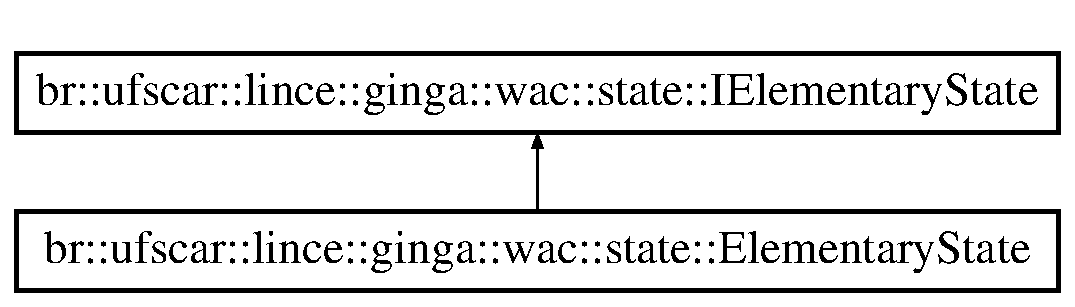
\includegraphics[height=2cm]{classbr_1_1ufscar_1_1lince_1_1ginga_1_1wac_1_1state_1_1ElementaryState}
\end{center}
\end{figure}
\subsection*{Public Member Functions}
\begin{DoxyCompactItemize}
\item 
virtual short \hyperlink{classbr_1_1ufscar_1_1lince_1_1ginga_1_1wac_1_1state_1_1ElementaryState_a08806ab0fedbb9684ca5a0d1cb42c5ac}{getStatus} ()
\begin{DoxyCompactList}\small\item\em Este método retorna uma número que representa o estado do player. \item\end{DoxyCompactList}\item 
virtual double \hyperlink{classbr_1_1ufscar_1_1lince_1_1ginga_1_1wac_1_1state_1_1ElementaryState_a05bc58afddd1713b6300f383b7e26826}{getMediaTime} ()
\begin{DoxyCompactList}\small\item\em Este método retorna o tempo atual do player, considerando o inicio como sendo 0. \item\end{DoxyCompactList}\item 
virtual int \hyperlink{classbr_1_1ufscar_1_1lince_1_1ginga_1_1wac_1_1state_1_1ElementaryState_afe5f10172203bf1bc6064166658de738}{getHight} ()
\begin{DoxyCompactList}\small\item\em Este método retorna a altura da imagem exibida pelo player. \item\end{DoxyCompactList}\item 
virtual int \hyperlink{classbr_1_1ufscar_1_1lince_1_1ginga_1_1wac_1_1state_1_1ElementaryState_adf39d11c81458c2b636b797821a81fc3}{getWidh} ()
\begin{DoxyCompactList}\small\item\em Este método retorna a largura da imagem exibida pelo player. \item\end{DoxyCompactList}\item 
virtual bool \hyperlink{classbr_1_1ufscar_1_1lince_1_1ginga_1_1wac_1_1state_1_1ElementaryState_ab247813eed9444dfb53c59235b1f91a9}{isPresented} ()
\begin{DoxyCompactList}\small\item\em Este permite saber se a apresentação do player já foi encerrada. \item\end{DoxyCompactList}\item 
virtual bool \hyperlink{classbr_1_1ufscar_1_1lince_1_1ginga_1_1wac_1_1state_1_1ElementaryState_a2e7a6f98a2b3a239f9b14f22025fc379}{isVisible} ()
\begin{DoxyCompactList}\small\item\em Este permite saber a mídia exibida pelo player está visivel. \item\end{DoxyCompactList}\item 
virtual string \hyperlink{classbr_1_1ufscar_1_1lince_1_1ginga_1_1wac_1_1state_1_1ElementaryState_aaa47390c93fda945f7ba5ee80031a137}{getPropertyValue} (string name)
\begin{DoxyCompactList}\small\item\em Este método permite obter o valor de uma propriedade do player. \item\end{DoxyCompactList}\item 
virtual vector$<$ string $>$ $\ast$ \hyperlink{classbr_1_1ufscar_1_1lince_1_1ginga_1_1wac_1_1state_1_1ElementaryState_a135050e832afa82aeff759a54087031b}{getPropertiesNames} ()
\begin{DoxyCompactList}\small\item\em Este método permite otbter todos os nomes das propriedades possuidas pelo player. \item\end{DoxyCompactList}\item 
virtual string \hyperlink{classbr_1_1ufscar_1_1lince_1_1ginga_1_1wac_1_1state_1_1ElementaryState_a3714512e115e6e66bfa55eb5694951ec}{getMrl} ()
\begin{DoxyCompactList}\small\item\em Este método permite obter o MRL da mídia executada pelo player. \item\end{DoxyCompactList}\item 
virtual string \hyperlink{classbr_1_1ufscar_1_1lince_1_1ginga_1_1wac_1_1state_1_1ElementaryState_ae1c2e7da72253acf9b5c19754994047c}{getStatusName} ()
\begin{DoxyCompactList}\small\item\em Este método retorna um string que representa o estado atual do player. \item\end{DoxyCompactList}\item 
\hyperlink{classbr_1_1ufscar_1_1lince_1_1ginga_1_1wac_1_1state_1_1ElementaryState_abd089616d40c13eb528a92984252a58f}{$\sim$ElementaryState} ()
\begin{DoxyCompactList}\small\item\em Destrutor. \item\end{DoxyCompactList}\item 
\hyperlink{classbr_1_1ufscar_1_1lince_1_1ginga_1_1wac_1_1state_1_1ElementaryState_ad47a64749c66f7257d36911ade24ea77}{ElementaryState} (PlayerState $\ast$playerState)
\begin{DoxyCompactList}\small\item\em Construtor. \item\end{DoxyCompactList}\end{DoxyCompactItemize}


\subsection{Detailed Description}
Esta classe generica representa o Estado de um Player em um determinado momento, servindo de interface com as aplicações que desejam obter os estados do player. Futuramente, ela pode ser espandida para armazenar mais informações referentes ao estado do player que não podem ser obtidas diretamente da módulo players, mas sim da classe PlayerAdapter do módulo Formatter. 

\subsection{Constructor \& Destructor Documentation}
\hypertarget{classbr_1_1ufscar_1_1lince_1_1ginga_1_1wac_1_1state_1_1ElementaryState_abd089616d40c13eb528a92984252a58f}{
\index{br::ufscar::lince::ginga::wac::state::ElementaryState@{br::ufscar::lince::ginga::wac::state::ElementaryState}!$\sim$ElementaryState@{$\sim$ElementaryState}}
\index{$\sim$ElementaryState@{$\sim$ElementaryState}!br::ufscar::lince::ginga::wac::state::ElementaryState@{br::ufscar::lince::ginga::wac::state::ElementaryState}}
\subsubsection[{$\sim$ElementaryState}]{\setlength{\rightskip}{0pt plus 5cm}br::ufscar::lince::ginga::wac::state::ElementaryState::$\sim$ElementaryState ()}}
\label{classbr_1_1ufscar_1_1lince_1_1ginga_1_1wac_1_1state_1_1ElementaryState_abd089616d40c13eb528a92984252a58f}


Destrutor. 

\hypertarget{classbr_1_1ufscar_1_1lince_1_1ginga_1_1wac_1_1state_1_1ElementaryState_ad47a64749c66f7257d36911ade24ea77}{
\index{br::ufscar::lince::ginga::wac::state::ElementaryState@{br::ufscar::lince::ginga::wac::state::ElementaryState}!ElementaryState@{ElementaryState}}
\index{ElementaryState@{ElementaryState}!br::ufscar::lince::ginga::wac::state::ElementaryState@{br::ufscar::lince::ginga::wac::state::ElementaryState}}
\subsubsection[{ElementaryState}]{\setlength{\rightskip}{0pt plus 5cm}br::ufscar::lince::ginga::wac::state::ElementaryState::ElementaryState (PlayerState $\ast$ {\em playerState})}}
\label{classbr_1_1ufscar_1_1lince_1_1ginga_1_1wac_1_1state_1_1ElementaryState_ad47a64749c66f7257d36911ade24ea77}


Construtor. 


\begin{DoxyParams}{Parameters}
\item[{\em playerState}]Instância que contém as informações relativas ao estado dos players. \end{DoxyParams}


\subsection{Member Function Documentation}
\hypertarget{classbr_1_1ufscar_1_1lince_1_1ginga_1_1wac_1_1state_1_1ElementaryState_afe5f10172203bf1bc6064166658de738}{
\index{br::ufscar::lince::ginga::wac::state::ElementaryState@{br::ufscar::lince::ginga::wac::state::ElementaryState}!getHight@{getHight}}
\index{getHight@{getHight}!br::ufscar::lince::ginga::wac::state::ElementaryState@{br::ufscar::lince::ginga::wac::state::ElementaryState}}
\subsubsection[{getHight}]{\setlength{\rightskip}{0pt plus 5cm}virtual int br::ufscar::lince::ginga::wac::state::ElementaryState::getHight ()\hspace{0.3cm}{\ttfamily  \mbox{[}virtual\mbox{]}}}}
\label{classbr_1_1ufscar_1_1lince_1_1ginga_1_1wac_1_1state_1_1ElementaryState_afe5f10172203bf1bc6064166658de738}


Este método retorna a altura da imagem exibida pelo player. 

\begin{DoxyReturn}{Returns}
Altura da Imagem exibida pelo player 
\end{DoxyReturn}


Implements \hyperlink{classbr_1_1ufscar_1_1lince_1_1ginga_1_1wac_1_1state_1_1IElementaryState_a22990483a86a4fdb0d8203c2f96f701c}{br::ufscar::lince::ginga::wac::state::IElementaryState}.

\hypertarget{classbr_1_1ufscar_1_1lince_1_1ginga_1_1wac_1_1state_1_1ElementaryState_a05bc58afddd1713b6300f383b7e26826}{
\index{br::ufscar::lince::ginga::wac::state::ElementaryState@{br::ufscar::lince::ginga::wac::state::ElementaryState}!getMediaTime@{getMediaTime}}
\index{getMediaTime@{getMediaTime}!br::ufscar::lince::ginga::wac::state::ElementaryState@{br::ufscar::lince::ginga::wac::state::ElementaryState}}
\subsubsection[{getMediaTime}]{\setlength{\rightskip}{0pt plus 5cm}virtual double br::ufscar::lince::ginga::wac::state::ElementaryState::getMediaTime ()\hspace{0.3cm}{\ttfamily  \mbox{[}virtual\mbox{]}}}}
\label{classbr_1_1ufscar_1_1lince_1_1ginga_1_1wac_1_1state_1_1ElementaryState_a05bc58afddd1713b6300f383b7e26826}


Este método retorna o tempo atual do player, considerando o inicio como sendo 0. 

\begin{DoxyReturn}{Returns}
O tempo atual do player. 
\end{DoxyReturn}


Implements \hyperlink{classbr_1_1ufscar_1_1lince_1_1ginga_1_1wac_1_1state_1_1IElementaryState_a2dd09dc8dcee4eb6a4b23fe4d1f001ad}{br::ufscar::lince::ginga::wac::state::IElementaryState}.

\hypertarget{classbr_1_1ufscar_1_1lince_1_1ginga_1_1wac_1_1state_1_1ElementaryState_a3714512e115e6e66bfa55eb5694951ec}{
\index{br::ufscar::lince::ginga::wac::state::ElementaryState@{br::ufscar::lince::ginga::wac::state::ElementaryState}!getMrl@{getMrl}}
\index{getMrl@{getMrl}!br::ufscar::lince::ginga::wac::state::ElementaryState@{br::ufscar::lince::ginga::wac::state::ElementaryState}}
\subsubsection[{getMrl}]{\setlength{\rightskip}{0pt plus 5cm}virtual string br::ufscar::lince::ginga::wac::state::ElementaryState::getMrl ()\hspace{0.3cm}{\ttfamily  \mbox{[}virtual\mbox{]}}}}
\label{classbr_1_1ufscar_1_1lince_1_1ginga_1_1wac_1_1state_1_1ElementaryState_a3714512e115e6e66bfa55eb5694951ec}


Este método permite obter o MRL da mídia executada pelo player. 

\begin{DoxyReturn}{Returns}
Mrl da mídia executada pelo player. 
\end{DoxyReturn}


Implements \hyperlink{classbr_1_1ufscar_1_1lince_1_1ginga_1_1wac_1_1state_1_1IElementaryState_a5fae9abe330000d369a739626d089a87}{br::ufscar::lince::ginga::wac::state::IElementaryState}.

\hypertarget{classbr_1_1ufscar_1_1lince_1_1ginga_1_1wac_1_1state_1_1ElementaryState_a135050e832afa82aeff759a54087031b}{
\index{br::ufscar::lince::ginga::wac::state::ElementaryState@{br::ufscar::lince::ginga::wac::state::ElementaryState}!getPropertiesNames@{getPropertiesNames}}
\index{getPropertiesNames@{getPropertiesNames}!br::ufscar::lince::ginga::wac::state::ElementaryState@{br::ufscar::lince::ginga::wac::state::ElementaryState}}
\subsubsection[{getPropertiesNames}]{\setlength{\rightskip}{0pt plus 5cm}virtual vector$<$string$>$$\ast$ br::ufscar::lince::ginga::wac::state::ElementaryState::getPropertiesNames ()\hspace{0.3cm}{\ttfamily  \mbox{[}virtual\mbox{]}}}}
\label{classbr_1_1ufscar_1_1lince_1_1ginga_1_1wac_1_1state_1_1ElementaryState_a135050e832afa82aeff759a54087031b}


Este método permite otbter todos os nomes das propriedades possuidas pelo player. 

\begin{DoxyReturn}{Returns}
Vetor contento todos os nomes das propriedades. 
\end{DoxyReturn}


Implements \hyperlink{classbr_1_1ufscar_1_1lince_1_1ginga_1_1wac_1_1state_1_1IElementaryState_a68c7e2ba58623cea860d6de1fc7112e7}{br::ufscar::lince::ginga::wac::state::IElementaryState}.

\hypertarget{classbr_1_1ufscar_1_1lince_1_1ginga_1_1wac_1_1state_1_1ElementaryState_aaa47390c93fda945f7ba5ee80031a137}{
\index{br::ufscar::lince::ginga::wac::state::ElementaryState@{br::ufscar::lince::ginga::wac::state::ElementaryState}!getPropertyValue@{getPropertyValue}}
\index{getPropertyValue@{getPropertyValue}!br::ufscar::lince::ginga::wac::state::ElementaryState@{br::ufscar::lince::ginga::wac::state::ElementaryState}}
\subsubsection[{getPropertyValue}]{\setlength{\rightskip}{0pt plus 5cm}virtual string br::ufscar::lince::ginga::wac::state::ElementaryState::getPropertyValue (string {\em name})\hspace{0.3cm}{\ttfamily  \mbox{[}virtual\mbox{]}}}}
\label{classbr_1_1ufscar_1_1lince_1_1ginga_1_1wac_1_1state_1_1ElementaryState_aaa47390c93fda945f7ba5ee80031a137}


Este método permite obter o valor de uma propriedade do player. 


\begin{DoxyParams}{Parameters}
\item[{\em name}]Nome da propriedade a ser obtida \end{DoxyParams}
\begin{DoxyReturn}{Returns}
Valor da propriedade armazenada em um string. 
\end{DoxyReturn}


Implements \hyperlink{classbr_1_1ufscar_1_1lince_1_1ginga_1_1wac_1_1state_1_1IElementaryState_a01bae35ea4efe31c179e81db8fb8a126}{br::ufscar::lince::ginga::wac::state::IElementaryState}.

\hypertarget{classbr_1_1ufscar_1_1lince_1_1ginga_1_1wac_1_1state_1_1ElementaryState_a08806ab0fedbb9684ca5a0d1cb42c5ac}{
\index{br::ufscar::lince::ginga::wac::state::ElementaryState@{br::ufscar::lince::ginga::wac::state::ElementaryState}!getStatus@{getStatus}}
\index{getStatus@{getStatus}!br::ufscar::lince::ginga::wac::state::ElementaryState@{br::ufscar::lince::ginga::wac::state::ElementaryState}}
\subsubsection[{getStatus}]{\setlength{\rightskip}{0pt plus 5cm}virtual short br::ufscar::lince::ginga::wac::state::ElementaryState::getStatus ()\hspace{0.3cm}{\ttfamily  \mbox{[}virtual\mbox{]}}}}
\label{classbr_1_1ufscar_1_1lince_1_1ginga_1_1wac_1_1state_1_1ElementaryState_a08806ab0fedbb9684ca5a0d1cb42c5ac}


Este método retorna uma número que representa o estado do player. 

\begin{DoxyReturn}{Returns}
Um número que representa o estado do player 
\end{DoxyReturn}


Implements \hyperlink{classbr_1_1ufscar_1_1lince_1_1ginga_1_1wac_1_1state_1_1IElementaryState_a6df6b08801327e6b2c06c428119caba9}{br::ufscar::lince::ginga::wac::state::IElementaryState}.

\hypertarget{classbr_1_1ufscar_1_1lince_1_1ginga_1_1wac_1_1state_1_1ElementaryState_ae1c2e7da72253acf9b5c19754994047c}{
\index{br::ufscar::lince::ginga::wac::state::ElementaryState@{br::ufscar::lince::ginga::wac::state::ElementaryState}!getStatusName@{getStatusName}}
\index{getStatusName@{getStatusName}!br::ufscar::lince::ginga::wac::state::ElementaryState@{br::ufscar::lince::ginga::wac::state::ElementaryState}}
\subsubsection[{getStatusName}]{\setlength{\rightskip}{0pt plus 5cm}virtual string br::ufscar::lince::ginga::wac::state::ElementaryState::getStatusName ()\hspace{0.3cm}{\ttfamily  \mbox{[}virtual\mbox{]}}}}
\label{classbr_1_1ufscar_1_1lince_1_1ginga_1_1wac_1_1state_1_1ElementaryState_ae1c2e7da72253acf9b5c19754994047c}


Este método retorna um string que representa o estado atual do player. 

Os nomes possíveis de serem retornados são: 'NOME', 'PLAY', 'PAUSE' e 'STOP' \begin{DoxyReturn}{Returns}
String com o nome do estado atual do player. 
\end{DoxyReturn}


Implements \hyperlink{classbr_1_1ufscar_1_1lince_1_1ginga_1_1wac_1_1state_1_1IElementaryState_abeabe720e157120f97d6a911460f6d71}{br::ufscar::lince::ginga::wac::state::IElementaryState}.

\hypertarget{classbr_1_1ufscar_1_1lince_1_1ginga_1_1wac_1_1state_1_1ElementaryState_adf39d11c81458c2b636b797821a81fc3}{
\index{br::ufscar::lince::ginga::wac::state::ElementaryState@{br::ufscar::lince::ginga::wac::state::ElementaryState}!getWidh@{getWidh}}
\index{getWidh@{getWidh}!br::ufscar::lince::ginga::wac::state::ElementaryState@{br::ufscar::lince::ginga::wac::state::ElementaryState}}
\subsubsection[{getWidh}]{\setlength{\rightskip}{0pt plus 5cm}virtual int br::ufscar::lince::ginga::wac::state::ElementaryState::getWidh ()\hspace{0.3cm}{\ttfamily  \mbox{[}virtual\mbox{]}}}}
\label{classbr_1_1ufscar_1_1lince_1_1ginga_1_1wac_1_1state_1_1ElementaryState_adf39d11c81458c2b636b797821a81fc3}


Este método retorna a largura da imagem exibida pelo player. 

\begin{DoxyReturn}{Returns}
Largura da Imagem exibida pelo player 
\end{DoxyReturn}


Implements \hyperlink{classbr_1_1ufscar_1_1lince_1_1ginga_1_1wac_1_1state_1_1IElementaryState_a13218fa1e799a3aabc8f20ffd7c134f5}{br::ufscar::lince::ginga::wac::state::IElementaryState}.

\hypertarget{classbr_1_1ufscar_1_1lince_1_1ginga_1_1wac_1_1state_1_1ElementaryState_ab247813eed9444dfb53c59235b1f91a9}{
\index{br::ufscar::lince::ginga::wac::state::ElementaryState@{br::ufscar::lince::ginga::wac::state::ElementaryState}!isPresented@{isPresented}}
\index{isPresented@{isPresented}!br::ufscar::lince::ginga::wac::state::ElementaryState@{br::ufscar::lince::ginga::wac::state::ElementaryState}}
\subsubsection[{isPresented}]{\setlength{\rightskip}{0pt plus 5cm}virtual bool br::ufscar::lince::ginga::wac::state::ElementaryState::isPresented ()\hspace{0.3cm}{\ttfamily  \mbox{[}virtual\mbox{]}}}}
\label{classbr_1_1ufscar_1_1lince_1_1ginga_1_1wac_1_1state_1_1ElementaryState_ab247813eed9444dfb53c59235b1f91a9}


Este permite saber se a apresentação do player já foi encerrada. 

\begin{DoxyReturn}{Returns}
True se a apresentação já foi encerrada; False caso contrário. 
\end{DoxyReturn}


Implements \hyperlink{classbr_1_1ufscar_1_1lince_1_1ginga_1_1wac_1_1state_1_1IElementaryState_a2d7a7f8c9945df9ad15d87863a1d288e}{br::ufscar::lince::ginga::wac::state::IElementaryState}.

\hypertarget{classbr_1_1ufscar_1_1lince_1_1ginga_1_1wac_1_1state_1_1ElementaryState_a2e7a6f98a2b3a239f9b14f22025fc379}{
\index{br::ufscar::lince::ginga::wac::state::ElementaryState@{br::ufscar::lince::ginga::wac::state::ElementaryState}!isVisible@{isVisible}}
\index{isVisible@{isVisible}!br::ufscar::lince::ginga::wac::state::ElementaryState@{br::ufscar::lince::ginga::wac::state::ElementaryState}}
\subsubsection[{isVisible}]{\setlength{\rightskip}{0pt plus 5cm}virtual bool br::ufscar::lince::ginga::wac::state::ElementaryState::isVisible ()\hspace{0.3cm}{\ttfamily  \mbox{[}virtual\mbox{]}}}}
\label{classbr_1_1ufscar_1_1lince_1_1ginga_1_1wac_1_1state_1_1ElementaryState_a2e7a6f98a2b3a239f9b14f22025fc379}


Este permite saber a mídia exibida pelo player está visivel. 

\begin{DoxyReturn}{Returns}
True se está visivel; False caso contrário. 
\end{DoxyReturn}


Implements \hyperlink{classbr_1_1ufscar_1_1lince_1_1ginga_1_1wac_1_1state_1_1IElementaryState_a64cd15f7d8434054345243d877ede453}{br::ufscar::lince::ginga::wac::state::IElementaryState}.



The documentation for this class was generated from the following file:\begin{DoxyCompactItemize}
\item 
include/\hyperlink{ElementaryState_8h}{ElementaryState.h}\end{DoxyCompactItemize}

\hypertarget{classbr_1_1ufscar_1_1lince_1_1ginga_1_1wac_1_1state_1_1IContextProvider}{
\section{br::ufscar::lince::ginga::wac::state::IContextProvider Class Reference}
\label{classbr_1_1ufscar_1_1lince_1_1ginga_1_1wac_1_1state_1_1IContextProvider}\index{br::ufscar::lince::ginga::wac::state::IContextProvider@{br::ufscar::lince::ginga::wac::state::IContextProvider}}
}


Esta classe virtual deve ser implementada por classes que são capazes de informar o contexto de uma apresentação NCL.  




{\ttfamily \#include $<$IContextProvider.h$>$}

\subsection*{Public Member Functions}
\begin{DoxyCompactItemize}
\item 
virtual \hyperlink{classbr_1_1ufscar_1_1lince_1_1ginga_1_1wac_1_1state_1_1IContextProvider_a586f6b390cf22fb589aa3b6fb661dc49}{$\sim$IContextProvider} ()
\begin{DoxyCompactList}\small\item\em Destrutor Genérico. \item\end{DoxyCompactList}\item 
virtual vector$<$ string $>$ $\ast$ \hyperlink{classbr_1_1ufscar_1_1lince_1_1ginga_1_1wac_1_1state_1_1IContextProvider_a1912620e1f978f7e12dba01b0c31af5c}{getPropertyNames} ()=0
\begin{DoxyCompactList}\small\item\em Este método é utilizado pelo \hyperlink{classbr_1_1ufscar_1_1lince_1_1ginga_1_1wac_1_1state_1_1StateManager}{StateManager} para obter os nomes das propriedades existentes no contexto da aplicação. \item\end{DoxyCompactList}\item 
virtual string \hyperlink{classbr_1_1ufscar_1_1lince_1_1ginga_1_1wac_1_1state_1_1IContextProvider_a0777035084d9b444f13b85b71cda6927}{getPropertyValue} (string attributeId)=0
\begin{DoxyCompactList}\small\item\em Este método é utilizado pelo \hyperlink{classbr_1_1ufscar_1_1lince_1_1ginga_1_1wac_1_1state_1_1StateManager}{StateManager} apra obter o valor das propriedades existentes no contexto da aplicação. \item\end{DoxyCompactList}\end{DoxyCompactItemize}


\subsection{Detailed Description}
Esta classe virtual deve ser implementada por classes que são capazes de informar o contexto de uma apresentação NCL. 

\subsection{Constructor \& Destructor Documentation}
\hypertarget{classbr_1_1ufscar_1_1lince_1_1ginga_1_1wac_1_1state_1_1IContextProvider_a586f6b390cf22fb589aa3b6fb661dc49}{
\index{br::ufscar::lince::ginga::wac::state::IContextProvider@{br::ufscar::lince::ginga::wac::state::IContextProvider}!$\sim$IContextProvider@{$\sim$IContextProvider}}
\index{$\sim$IContextProvider@{$\sim$IContextProvider}!br::ufscar::lince::ginga::wac::state::IContextProvider@{br::ufscar::lince::ginga::wac::state::IContextProvider}}
\subsubsection[{$\sim$IContextProvider}]{\setlength{\rightskip}{0pt plus 5cm}virtual br::ufscar::lince::ginga::wac::state::IContextProvider::$\sim$IContextProvider ()\hspace{0.3cm}{\ttfamily  \mbox{[}inline, virtual\mbox{]}}}}
\label{classbr_1_1ufscar_1_1lince_1_1ginga_1_1wac_1_1state_1_1IContextProvider_a586f6b390cf22fb589aa3b6fb661dc49}


Destrutor Genérico. 



\subsection{Member Function Documentation}
\hypertarget{classbr_1_1ufscar_1_1lince_1_1ginga_1_1wac_1_1state_1_1IContextProvider_a1912620e1f978f7e12dba01b0c31af5c}{
\index{br::ufscar::lince::ginga::wac::state::IContextProvider@{br::ufscar::lince::ginga::wac::state::IContextProvider}!getPropertyNames@{getPropertyNames}}
\index{getPropertyNames@{getPropertyNames}!br::ufscar::lince::ginga::wac::state::IContextProvider@{br::ufscar::lince::ginga::wac::state::IContextProvider}}
\subsubsection[{getPropertyNames}]{\setlength{\rightskip}{0pt plus 5cm}virtual vector$<$string$>$$\ast$ br::ufscar::lince::ginga::wac::state::IContextProvider::getPropertyNames ()\hspace{0.3cm}{\ttfamily  \mbox{[}pure virtual\mbox{]}}}}
\label{classbr_1_1ufscar_1_1lince_1_1ginga_1_1wac_1_1state_1_1IContextProvider_a1912620e1f978f7e12dba01b0c31af5c}


Este método é utilizado pelo \hyperlink{classbr_1_1ufscar_1_1lince_1_1ginga_1_1wac_1_1state_1_1StateManager}{StateManager} para obter os nomes das propriedades existentes no contexto da aplicação. 

\begin{DoxyReturn}{Returns}
Um vetor contento os nomes das propriedades existentes no contexto da aplicação 
\end{DoxyReturn}
\hypertarget{classbr_1_1ufscar_1_1lince_1_1ginga_1_1wac_1_1state_1_1IContextProvider_a0777035084d9b444f13b85b71cda6927}{
\index{br::ufscar::lince::ginga::wac::state::IContextProvider@{br::ufscar::lince::ginga::wac::state::IContextProvider}!getPropertyValue@{getPropertyValue}}
\index{getPropertyValue@{getPropertyValue}!br::ufscar::lince::ginga::wac::state::IContextProvider@{br::ufscar::lince::ginga::wac::state::IContextProvider}}
\subsubsection[{getPropertyValue}]{\setlength{\rightskip}{0pt plus 5cm}virtual string br::ufscar::lince::ginga::wac::state::IContextProvider::getPropertyValue (string {\em attributeId})\hspace{0.3cm}{\ttfamily  \mbox{[}pure virtual\mbox{]}}}}
\label{classbr_1_1ufscar_1_1lince_1_1ginga_1_1wac_1_1state_1_1IContextProvider_a0777035084d9b444f13b85b71cda6927}


Este método é utilizado pelo \hyperlink{classbr_1_1ufscar_1_1lince_1_1ginga_1_1wac_1_1state_1_1StateManager}{StateManager} apra obter o valor das propriedades existentes no contexto da aplicação. 


\begin{DoxyParams}{Parameters}
\item[{\em attributeId}]Nome da propriedade da qual o valor será recuperado. \end{DoxyParams}
\begin{DoxyReturn}{Returns}
Valor da propriedade representado através de um string. 
\end{DoxyReturn}


The documentation for this class was generated from the following file:\begin{DoxyCompactItemize}
\item 
include/\hyperlink{IContextProvider_8h}{IContextProvider.h}\end{DoxyCompactItemize}

\hypertarget{classbr_1_1ufscar_1_1lince_1_1ginga_1_1wac_1_1state_1_1IElementaryState}{
\section{br::ufscar::lince::ginga::wac::state::IElementaryState Class Reference}
\label{classbr_1_1ufscar_1_1lince_1_1ginga_1_1wac_1_1state_1_1IElementaryState}\index{br::ufscar::lince::ginga::wac::state::IElementaryState@{br::ufscar::lince::ginga::wac::state::IElementaryState}}
}


Esta classe generica representa o Estado de um Player em um determinado momento, servindo de interface com as aplicações que desejam obter os estados do player.  




{\ttfamily \#include $<$IElementaryState.h$>$}

Inheritance diagram for br::ufscar::lince::ginga::wac::state::IElementaryState:\begin{figure}[H]
\begin{center}
\leavevmode
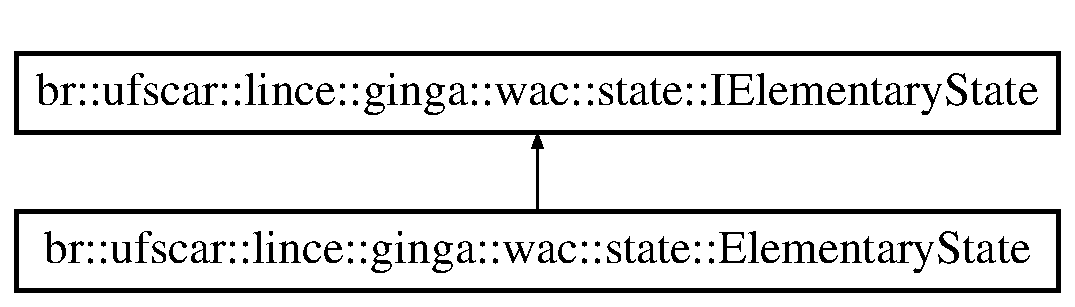
\includegraphics[height=2cm]{classbr_1_1ufscar_1_1lince_1_1ginga_1_1wac_1_1state_1_1IElementaryState}
\end{center}
\end{figure}
\subsection*{Public Member Functions}
\begin{DoxyCompactItemize}
\item 
virtual short \hyperlink{classbr_1_1ufscar_1_1lince_1_1ginga_1_1wac_1_1state_1_1IElementaryState_a6df6b08801327e6b2c06c428119caba9}{getStatus} ()=0
\begin{DoxyCompactList}\small\item\em Este método retorna uma número que representa o estado do player. \item\end{DoxyCompactList}\item 
virtual double \hyperlink{classbr_1_1ufscar_1_1lince_1_1ginga_1_1wac_1_1state_1_1IElementaryState_a2dd09dc8dcee4eb6a4b23fe4d1f001ad}{getMediaTime} ()=0
\begin{DoxyCompactList}\small\item\em Este método retorna o tempo atual do player, considerando o inicio como sendo 0. \item\end{DoxyCompactList}\item 
virtual int \hyperlink{classbr_1_1ufscar_1_1lince_1_1ginga_1_1wac_1_1state_1_1IElementaryState_a22990483a86a4fdb0d8203c2f96f701c}{getHight} ()=0
\begin{DoxyCompactList}\small\item\em Este método retorna a altura da imagem exibida pelo player. \item\end{DoxyCompactList}\item 
virtual int \hyperlink{classbr_1_1ufscar_1_1lince_1_1ginga_1_1wac_1_1state_1_1IElementaryState_a13218fa1e799a3aabc8f20ffd7c134f5}{getWidh} ()=0
\begin{DoxyCompactList}\small\item\em Este método retorna a largura da imagem exibida pelo player. \item\end{DoxyCompactList}\item 
virtual bool \hyperlink{classbr_1_1ufscar_1_1lince_1_1ginga_1_1wac_1_1state_1_1IElementaryState_a2d7a7f8c9945df9ad15d87863a1d288e}{isPresented} ()=0
\begin{DoxyCompactList}\small\item\em Este permite saber se a apresentação do player já foi encerrada. \item\end{DoxyCompactList}\item 
virtual bool \hyperlink{classbr_1_1ufscar_1_1lince_1_1ginga_1_1wac_1_1state_1_1IElementaryState_a64cd15f7d8434054345243d877ede453}{isVisible} ()=0
\begin{DoxyCompactList}\small\item\em Este permite saber a mídia exibida pelo player está visivel. \item\end{DoxyCompactList}\item 
virtual string \hyperlink{classbr_1_1ufscar_1_1lince_1_1ginga_1_1wac_1_1state_1_1IElementaryState_a01bae35ea4efe31c179e81db8fb8a126}{getPropertyValue} (string name)=0
\begin{DoxyCompactList}\small\item\em Este método permite obter o valor de uma propriedade do player. \item\end{DoxyCompactList}\item 
virtual vector$<$ string $>$ $\ast$ \hyperlink{classbr_1_1ufscar_1_1lince_1_1ginga_1_1wac_1_1state_1_1IElementaryState_a68c7e2ba58623cea860d6de1fc7112e7}{getPropertiesNames} ()=0
\begin{DoxyCompactList}\small\item\em Este método permite otbter todos os nomes das propriedades possuidas pelo player. \item\end{DoxyCompactList}\item 
virtual string \hyperlink{classbr_1_1ufscar_1_1lince_1_1ginga_1_1wac_1_1state_1_1IElementaryState_a5fae9abe330000d369a739626d089a87}{getMrl} ()=0
\begin{DoxyCompactList}\small\item\em Este método permite obter o MRL da mídia executada pelo player. \item\end{DoxyCompactList}\item 
virtual string \hyperlink{classbr_1_1ufscar_1_1lince_1_1ginga_1_1wac_1_1state_1_1IElementaryState_abeabe720e157120f97d6a911460f6d71}{getStatusName} ()=0
\begin{DoxyCompactList}\small\item\em Este método retorna um string que representa o estado atual do player. \item\end{DoxyCompactList}\item 
virtual \hyperlink{classbr_1_1ufscar_1_1lince_1_1ginga_1_1wac_1_1state_1_1IElementaryState_ae16e3a178e9c9b147bc0a02b5ddaf4e6}{$\sim$IElementaryState} ()
\begin{DoxyCompactList}\small\item\em Destrutor genérico. \item\end{DoxyCompactList}\end{DoxyCompactItemize}
\subsection*{Static Public Attributes}
\begin{DoxyCompactItemize}
\item 
static const short \hyperlink{classbr_1_1ufscar_1_1lince_1_1ginga_1_1wac_1_1state_1_1IElementaryState_a6b21cf3f8015ef6cbb839a2fc37e5a85}{NONE}
\begin{DoxyCompactList}\small\item\em Constante que representa o estado \char`\"{}nenhum\char`\"{} do player. \item\end{DoxyCompactList}\item 
static const short \hyperlink{classbr_1_1ufscar_1_1lince_1_1ginga_1_1wac_1_1state_1_1IElementaryState_a2d598e7badbbbb5460ed5e8204bb878f}{PLAY}
\begin{DoxyCompactList}\small\item\em Constante que representa o estado \char`\"{}em execução\char`\"{} do player. \item\end{DoxyCompactList}\item 
static const short \hyperlink{classbr_1_1ufscar_1_1lince_1_1ginga_1_1wac_1_1state_1_1IElementaryState_a66848654431dc226cdd3349f0aa845f1}{PAUSE}
\begin{DoxyCompactList}\small\item\em Constante que representa o estado \char`\"{}pausado\char`\"{} do player. \item\end{DoxyCompactList}\item 
static const short \hyperlink{classbr_1_1ufscar_1_1lince_1_1ginga_1_1wac_1_1state_1_1IElementaryState_af53fab5b92d73acc4fb6541d2906d6ce}{STOP}
\begin{DoxyCompactList}\small\item\em Constante que representa o estado \char`\"{}parado\char`\"{} do player. \item\end{DoxyCompactList}\end{DoxyCompactItemize}


\subsection{Detailed Description}
Esta classe generica representa o Estado de um Player em um determinado momento, servindo de interface com as aplicações que desejam obter os estados do player. Futuramente, ela pode ser espandida para armazenar mais informações referentes ao estado do player que não podem ser obtidas diretamente da módulo players, mas sim da classe PlayerAdapter do módulo Formatter. 

\subsection{Constructor \& Destructor Documentation}
\hypertarget{classbr_1_1ufscar_1_1lince_1_1ginga_1_1wac_1_1state_1_1IElementaryState_ae16e3a178e9c9b147bc0a02b5ddaf4e6}{
\index{br::ufscar::lince::ginga::wac::state::IElementaryState@{br::ufscar::lince::ginga::wac::state::IElementaryState}!$\sim$IElementaryState@{$\sim$IElementaryState}}
\index{$\sim$IElementaryState@{$\sim$IElementaryState}!br::ufscar::lince::ginga::wac::state::IElementaryState@{br::ufscar::lince::ginga::wac::state::IElementaryState}}
\subsubsection[{$\sim$IElementaryState}]{\setlength{\rightskip}{0pt plus 5cm}virtual br::ufscar::lince::ginga::wac::state::IElementaryState::$\sim$IElementaryState ()\hspace{0.3cm}{\ttfamily  \mbox{[}inline, virtual\mbox{]}}}}
\label{classbr_1_1ufscar_1_1lince_1_1ginga_1_1wac_1_1state_1_1IElementaryState_ae16e3a178e9c9b147bc0a02b5ddaf4e6}


Destrutor genérico. 



\subsection{Member Function Documentation}
\hypertarget{classbr_1_1ufscar_1_1lince_1_1ginga_1_1wac_1_1state_1_1IElementaryState_a22990483a86a4fdb0d8203c2f96f701c}{
\index{br::ufscar::lince::ginga::wac::state::IElementaryState@{br::ufscar::lince::ginga::wac::state::IElementaryState}!getHight@{getHight}}
\index{getHight@{getHight}!br::ufscar::lince::ginga::wac::state::IElementaryState@{br::ufscar::lince::ginga::wac::state::IElementaryState}}
\subsubsection[{getHight}]{\setlength{\rightskip}{0pt plus 5cm}virtual int br::ufscar::lince::ginga::wac::state::IElementaryState::getHight ()\hspace{0.3cm}{\ttfamily  \mbox{[}pure virtual\mbox{]}}}}
\label{classbr_1_1ufscar_1_1lince_1_1ginga_1_1wac_1_1state_1_1IElementaryState_a22990483a86a4fdb0d8203c2f96f701c}


Este método retorna a altura da imagem exibida pelo player. 

\begin{DoxyReturn}{Returns}
Altura da Imagem exibida pelo player 
\end{DoxyReturn}


Implemented in \hyperlink{classbr_1_1ufscar_1_1lince_1_1ginga_1_1wac_1_1state_1_1ElementaryState_afe5f10172203bf1bc6064166658de738}{br::ufscar::lince::ginga::wac::state::ElementaryState}.

\hypertarget{classbr_1_1ufscar_1_1lince_1_1ginga_1_1wac_1_1state_1_1IElementaryState_a2dd09dc8dcee4eb6a4b23fe4d1f001ad}{
\index{br::ufscar::lince::ginga::wac::state::IElementaryState@{br::ufscar::lince::ginga::wac::state::IElementaryState}!getMediaTime@{getMediaTime}}
\index{getMediaTime@{getMediaTime}!br::ufscar::lince::ginga::wac::state::IElementaryState@{br::ufscar::lince::ginga::wac::state::IElementaryState}}
\subsubsection[{getMediaTime}]{\setlength{\rightskip}{0pt plus 5cm}virtual double br::ufscar::lince::ginga::wac::state::IElementaryState::getMediaTime ()\hspace{0.3cm}{\ttfamily  \mbox{[}pure virtual\mbox{]}}}}
\label{classbr_1_1ufscar_1_1lince_1_1ginga_1_1wac_1_1state_1_1IElementaryState_a2dd09dc8dcee4eb6a4b23fe4d1f001ad}


Este método retorna o tempo atual do player, considerando o inicio como sendo 0. 

\begin{DoxyReturn}{Returns}
O tempo atual do player. 
\end{DoxyReturn}


Implemented in \hyperlink{classbr_1_1ufscar_1_1lince_1_1ginga_1_1wac_1_1state_1_1ElementaryState_a05bc58afddd1713b6300f383b7e26826}{br::ufscar::lince::ginga::wac::state::ElementaryState}.

\hypertarget{classbr_1_1ufscar_1_1lince_1_1ginga_1_1wac_1_1state_1_1IElementaryState_a5fae9abe330000d369a739626d089a87}{
\index{br::ufscar::lince::ginga::wac::state::IElementaryState@{br::ufscar::lince::ginga::wac::state::IElementaryState}!getMrl@{getMrl}}
\index{getMrl@{getMrl}!br::ufscar::lince::ginga::wac::state::IElementaryState@{br::ufscar::lince::ginga::wac::state::IElementaryState}}
\subsubsection[{getMrl}]{\setlength{\rightskip}{0pt plus 5cm}virtual string br::ufscar::lince::ginga::wac::state::IElementaryState::getMrl ()\hspace{0.3cm}{\ttfamily  \mbox{[}pure virtual\mbox{]}}}}
\label{classbr_1_1ufscar_1_1lince_1_1ginga_1_1wac_1_1state_1_1IElementaryState_a5fae9abe330000d369a739626d089a87}


Este método permite obter o MRL da mídia executada pelo player. 

\begin{DoxyReturn}{Returns}
Mrl da mídia executada pelo player. 
\end{DoxyReturn}


Implemented in \hyperlink{classbr_1_1ufscar_1_1lince_1_1ginga_1_1wac_1_1state_1_1ElementaryState_a3714512e115e6e66bfa55eb5694951ec}{br::ufscar::lince::ginga::wac::state::ElementaryState}.

\hypertarget{classbr_1_1ufscar_1_1lince_1_1ginga_1_1wac_1_1state_1_1IElementaryState_a68c7e2ba58623cea860d6de1fc7112e7}{
\index{br::ufscar::lince::ginga::wac::state::IElementaryState@{br::ufscar::lince::ginga::wac::state::IElementaryState}!getPropertiesNames@{getPropertiesNames}}
\index{getPropertiesNames@{getPropertiesNames}!br::ufscar::lince::ginga::wac::state::IElementaryState@{br::ufscar::lince::ginga::wac::state::IElementaryState}}
\subsubsection[{getPropertiesNames}]{\setlength{\rightskip}{0pt plus 5cm}virtual vector$<$string$>$$\ast$ br::ufscar::lince::ginga::wac::state::IElementaryState::getPropertiesNames ()\hspace{0.3cm}{\ttfamily  \mbox{[}pure virtual\mbox{]}}}}
\label{classbr_1_1ufscar_1_1lince_1_1ginga_1_1wac_1_1state_1_1IElementaryState_a68c7e2ba58623cea860d6de1fc7112e7}


Este método permite otbter todos os nomes das propriedades possuidas pelo player. 

\begin{DoxyReturn}{Returns}
Vetor contento todos os nomes das propriedades. 
\end{DoxyReturn}


Implemented in \hyperlink{classbr_1_1ufscar_1_1lince_1_1ginga_1_1wac_1_1state_1_1ElementaryState_a135050e832afa82aeff759a54087031b}{br::ufscar::lince::ginga::wac::state::ElementaryState}.

\hypertarget{classbr_1_1ufscar_1_1lince_1_1ginga_1_1wac_1_1state_1_1IElementaryState_a01bae35ea4efe31c179e81db8fb8a126}{
\index{br::ufscar::lince::ginga::wac::state::IElementaryState@{br::ufscar::lince::ginga::wac::state::IElementaryState}!getPropertyValue@{getPropertyValue}}
\index{getPropertyValue@{getPropertyValue}!br::ufscar::lince::ginga::wac::state::IElementaryState@{br::ufscar::lince::ginga::wac::state::IElementaryState}}
\subsubsection[{getPropertyValue}]{\setlength{\rightskip}{0pt plus 5cm}virtual string br::ufscar::lince::ginga::wac::state::IElementaryState::getPropertyValue (string {\em name})\hspace{0.3cm}{\ttfamily  \mbox{[}pure virtual\mbox{]}}}}
\label{classbr_1_1ufscar_1_1lince_1_1ginga_1_1wac_1_1state_1_1IElementaryState_a01bae35ea4efe31c179e81db8fb8a126}


Este método permite obter o valor de uma propriedade do player. 


\begin{DoxyParams}{Parameters}
\item[{\em name}]Nome da propriedade a ser obtida \end{DoxyParams}
\begin{DoxyReturn}{Returns}
Valor da propriedade armazenada em um string. 
\end{DoxyReturn}


Implemented in \hyperlink{classbr_1_1ufscar_1_1lince_1_1ginga_1_1wac_1_1state_1_1ElementaryState_aaa47390c93fda945f7ba5ee80031a137}{br::ufscar::lince::ginga::wac::state::ElementaryState}.

\hypertarget{classbr_1_1ufscar_1_1lince_1_1ginga_1_1wac_1_1state_1_1IElementaryState_a6df6b08801327e6b2c06c428119caba9}{
\index{br::ufscar::lince::ginga::wac::state::IElementaryState@{br::ufscar::lince::ginga::wac::state::IElementaryState}!getStatus@{getStatus}}
\index{getStatus@{getStatus}!br::ufscar::lince::ginga::wac::state::IElementaryState@{br::ufscar::lince::ginga::wac::state::IElementaryState}}
\subsubsection[{getStatus}]{\setlength{\rightskip}{0pt plus 5cm}virtual short br::ufscar::lince::ginga::wac::state::IElementaryState::getStatus ()\hspace{0.3cm}{\ttfamily  \mbox{[}pure virtual\mbox{]}}}}
\label{classbr_1_1ufscar_1_1lince_1_1ginga_1_1wac_1_1state_1_1IElementaryState_a6df6b08801327e6b2c06c428119caba9}


Este método retorna uma número que representa o estado do player. 

\begin{DoxyReturn}{Returns}
Um número que representa o estado do player 
\end{DoxyReturn}


Implemented in \hyperlink{classbr_1_1ufscar_1_1lince_1_1ginga_1_1wac_1_1state_1_1ElementaryState_a08806ab0fedbb9684ca5a0d1cb42c5ac}{br::ufscar::lince::ginga::wac::state::ElementaryState}.

\hypertarget{classbr_1_1ufscar_1_1lince_1_1ginga_1_1wac_1_1state_1_1IElementaryState_abeabe720e157120f97d6a911460f6d71}{
\index{br::ufscar::lince::ginga::wac::state::IElementaryState@{br::ufscar::lince::ginga::wac::state::IElementaryState}!getStatusName@{getStatusName}}
\index{getStatusName@{getStatusName}!br::ufscar::lince::ginga::wac::state::IElementaryState@{br::ufscar::lince::ginga::wac::state::IElementaryState}}
\subsubsection[{getStatusName}]{\setlength{\rightskip}{0pt plus 5cm}virtual string br::ufscar::lince::ginga::wac::state::IElementaryState::getStatusName ()\hspace{0.3cm}{\ttfamily  \mbox{[}pure virtual\mbox{]}}}}
\label{classbr_1_1ufscar_1_1lince_1_1ginga_1_1wac_1_1state_1_1IElementaryState_abeabe720e157120f97d6a911460f6d71}


Este método retorna um string que representa o estado atual do player. 

Os nomes possíveis de serem retornados são: 'NOME', 'PLAY', 'PAUSE' e 'STOP' \begin{DoxyReturn}{Returns}
String com o nome do estado atual do player. 
\end{DoxyReturn}


Implemented in \hyperlink{classbr_1_1ufscar_1_1lince_1_1ginga_1_1wac_1_1state_1_1ElementaryState_ae1c2e7da72253acf9b5c19754994047c}{br::ufscar::lince::ginga::wac::state::ElementaryState}.

\hypertarget{classbr_1_1ufscar_1_1lince_1_1ginga_1_1wac_1_1state_1_1IElementaryState_a13218fa1e799a3aabc8f20ffd7c134f5}{
\index{br::ufscar::lince::ginga::wac::state::IElementaryState@{br::ufscar::lince::ginga::wac::state::IElementaryState}!getWidh@{getWidh}}
\index{getWidh@{getWidh}!br::ufscar::lince::ginga::wac::state::IElementaryState@{br::ufscar::lince::ginga::wac::state::IElementaryState}}
\subsubsection[{getWidh}]{\setlength{\rightskip}{0pt plus 5cm}virtual int br::ufscar::lince::ginga::wac::state::IElementaryState::getWidh ()\hspace{0.3cm}{\ttfamily  \mbox{[}pure virtual\mbox{]}}}}
\label{classbr_1_1ufscar_1_1lince_1_1ginga_1_1wac_1_1state_1_1IElementaryState_a13218fa1e799a3aabc8f20ffd7c134f5}


Este método retorna a largura da imagem exibida pelo player. 

\begin{DoxyReturn}{Returns}
Largura da Imagem exibida pelo player 
\end{DoxyReturn}


Implemented in \hyperlink{classbr_1_1ufscar_1_1lince_1_1ginga_1_1wac_1_1state_1_1ElementaryState_adf39d11c81458c2b636b797821a81fc3}{br::ufscar::lince::ginga::wac::state::ElementaryState}.

\hypertarget{classbr_1_1ufscar_1_1lince_1_1ginga_1_1wac_1_1state_1_1IElementaryState_a2d7a7f8c9945df9ad15d87863a1d288e}{
\index{br::ufscar::lince::ginga::wac::state::IElementaryState@{br::ufscar::lince::ginga::wac::state::IElementaryState}!isPresented@{isPresented}}
\index{isPresented@{isPresented}!br::ufscar::lince::ginga::wac::state::IElementaryState@{br::ufscar::lince::ginga::wac::state::IElementaryState}}
\subsubsection[{isPresented}]{\setlength{\rightskip}{0pt plus 5cm}virtual bool br::ufscar::lince::ginga::wac::state::IElementaryState::isPresented ()\hspace{0.3cm}{\ttfamily  \mbox{[}pure virtual\mbox{]}}}}
\label{classbr_1_1ufscar_1_1lince_1_1ginga_1_1wac_1_1state_1_1IElementaryState_a2d7a7f8c9945df9ad15d87863a1d288e}


Este permite saber se a apresentação do player já foi encerrada. 

\begin{DoxyReturn}{Returns}
True se a apresentação já foi encerrada; False caso contrário. 
\end{DoxyReturn}


Implemented in \hyperlink{classbr_1_1ufscar_1_1lince_1_1ginga_1_1wac_1_1state_1_1ElementaryState_ab247813eed9444dfb53c59235b1f91a9}{br::ufscar::lince::ginga::wac::state::ElementaryState}.

\hypertarget{classbr_1_1ufscar_1_1lince_1_1ginga_1_1wac_1_1state_1_1IElementaryState_a64cd15f7d8434054345243d877ede453}{
\index{br::ufscar::lince::ginga::wac::state::IElementaryState@{br::ufscar::lince::ginga::wac::state::IElementaryState}!isVisible@{isVisible}}
\index{isVisible@{isVisible}!br::ufscar::lince::ginga::wac::state::IElementaryState@{br::ufscar::lince::ginga::wac::state::IElementaryState}}
\subsubsection[{isVisible}]{\setlength{\rightskip}{0pt plus 5cm}virtual bool br::ufscar::lince::ginga::wac::state::IElementaryState::isVisible ()\hspace{0.3cm}{\ttfamily  \mbox{[}pure virtual\mbox{]}}}}
\label{classbr_1_1ufscar_1_1lince_1_1ginga_1_1wac_1_1state_1_1IElementaryState_a64cd15f7d8434054345243d877ede453}


Este permite saber a mídia exibida pelo player está visivel. 

\begin{DoxyReturn}{Returns}
True se está visivel; False caso contrário. 
\end{DoxyReturn}


Implemented in \hyperlink{classbr_1_1ufscar_1_1lince_1_1ginga_1_1wac_1_1state_1_1ElementaryState_a2e7a6f98a2b3a239f9b14f22025fc379}{br::ufscar::lince::ginga::wac::state::ElementaryState}.



\subsection{Field Documentation}
\hypertarget{classbr_1_1ufscar_1_1lince_1_1ginga_1_1wac_1_1state_1_1IElementaryState_a6b21cf3f8015ef6cbb839a2fc37e5a85}{
\index{br::ufscar::lince::ginga::wac::state::IElementaryState@{br::ufscar::lince::ginga::wac::state::IElementaryState}!NONE@{NONE}}
\index{NONE@{NONE}!br::ufscar::lince::ginga::wac::state::IElementaryState@{br::ufscar::lince::ginga::wac::state::IElementaryState}}
\subsubsection[{NONE}]{\setlength{\rightskip}{0pt plus 5cm}const short {\bf br::ufscar::lince::ginga::wac::state::IElementaryState::NONE}\hspace{0.3cm}{\ttfamily  \mbox{[}static\mbox{]}}}}
\label{classbr_1_1ufscar_1_1lince_1_1ginga_1_1wac_1_1state_1_1IElementaryState_a6b21cf3f8015ef6cbb839a2fc37e5a85}


Constante que representa o estado \char`\"{}nenhum\char`\"{} do player. 

\hypertarget{classbr_1_1ufscar_1_1lince_1_1ginga_1_1wac_1_1state_1_1IElementaryState_a66848654431dc226cdd3349f0aa845f1}{
\index{br::ufscar::lince::ginga::wac::state::IElementaryState@{br::ufscar::lince::ginga::wac::state::IElementaryState}!PAUSE@{PAUSE}}
\index{PAUSE@{PAUSE}!br::ufscar::lince::ginga::wac::state::IElementaryState@{br::ufscar::lince::ginga::wac::state::IElementaryState}}
\subsubsection[{PAUSE}]{\setlength{\rightskip}{0pt plus 5cm}const short {\bf br::ufscar::lince::ginga::wac::state::IElementaryState::PAUSE}\hspace{0.3cm}{\ttfamily  \mbox{[}static\mbox{]}}}}
\label{classbr_1_1ufscar_1_1lince_1_1ginga_1_1wac_1_1state_1_1IElementaryState_a66848654431dc226cdd3349f0aa845f1}


Constante que representa o estado \char`\"{}pausado\char`\"{} do player. 

\hypertarget{classbr_1_1ufscar_1_1lince_1_1ginga_1_1wac_1_1state_1_1IElementaryState_a2d598e7badbbbb5460ed5e8204bb878f}{
\index{br::ufscar::lince::ginga::wac::state::IElementaryState@{br::ufscar::lince::ginga::wac::state::IElementaryState}!PLAY@{PLAY}}
\index{PLAY@{PLAY}!br::ufscar::lince::ginga::wac::state::IElementaryState@{br::ufscar::lince::ginga::wac::state::IElementaryState}}
\subsubsection[{PLAY}]{\setlength{\rightskip}{0pt plus 5cm}const short {\bf br::ufscar::lince::ginga::wac::state::IElementaryState::PLAY}\hspace{0.3cm}{\ttfamily  \mbox{[}static\mbox{]}}}}
\label{classbr_1_1ufscar_1_1lince_1_1ginga_1_1wac_1_1state_1_1IElementaryState_a2d598e7badbbbb5460ed5e8204bb878f}


Constante que representa o estado \char`\"{}em execução\char`\"{} do player. 

\hypertarget{classbr_1_1ufscar_1_1lince_1_1ginga_1_1wac_1_1state_1_1IElementaryState_af53fab5b92d73acc4fb6541d2906d6ce}{
\index{br::ufscar::lince::ginga::wac::state::IElementaryState@{br::ufscar::lince::ginga::wac::state::IElementaryState}!STOP@{STOP}}
\index{STOP@{STOP}!br::ufscar::lince::ginga::wac::state::IElementaryState@{br::ufscar::lince::ginga::wac::state::IElementaryState}}
\subsubsection[{STOP}]{\setlength{\rightskip}{0pt plus 5cm}const short {\bf br::ufscar::lince::ginga::wac::state::IElementaryState::STOP}\hspace{0.3cm}{\ttfamily  \mbox{[}static\mbox{]}}}}
\label{classbr_1_1ufscar_1_1lince_1_1ginga_1_1wac_1_1state_1_1IElementaryState_af53fab5b92d73acc4fb6541d2906d6ce}


Constante que representa o estado \char`\"{}parado\char`\"{} do player. 



The documentation for this class was generated from the following file:\begin{DoxyCompactItemize}
\item 
include/\hyperlink{IElementaryState_8h}{IElementaryState.h}\end{DoxyCompactItemize}

\hypertarget{classbr_1_1ufscar_1_1lince_1_1ginga_1_1wac_1_1state_1_1IPresentationState}{
\section{br::ufscar::lince::ginga::wac::state::IPresentationState Class Reference}
\label{classbr_1_1ufscar_1_1lince_1_1ginga_1_1wac_1_1state_1_1IPresentationState}\index{br::ufscar::lince::ginga::wac::state::IPresentationState@{br::ufscar::lince::ginga::wac::state::IPresentationState}}
}


Esta classe genérica serve de interface como as apliações que desejam obter informações sobre o estado da aplicação.  




{\ttfamily \#include $<$IPresentationState.h$>$}

Inheritance diagram for br::ufscar::lince::ginga::wac::state::IPresentationState:\begin{figure}[H]
\begin{center}
\leavevmode
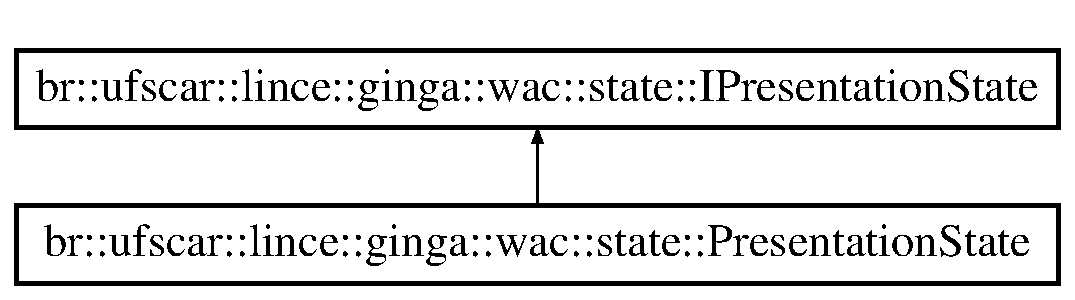
\includegraphics[height=2cm]{classbr_1_1ufscar_1_1lince_1_1ginga_1_1wac_1_1state_1_1IPresentationState}
\end{center}
\end{figure}
\subsection*{Public Member Functions}
\begin{DoxyCompactItemize}
\item 
\hyperlink{classbr_1_1ufscar_1_1lince_1_1ginga_1_1wac_1_1state_1_1IPresentationState_a4e3e2eac0d45ddcf17526115f9a7ef84}{$\sim$IPresentationState} ()
\item 
virtual vector$<$ string $>$ $\ast$ \hyperlink{classbr_1_1ufscar_1_1lince_1_1ginga_1_1wac_1_1state_1_1IPresentationState_ac3ba6e82191af041b1bc4320ddaf0ca5}{getPlayersNames} ()=0
\begin{DoxyCompactList}\small\item\em Retorna o nome de todos os players da apresentação atual. \item\end{DoxyCompactList}\item 
virtual \hyperlink{classbr_1_1ufscar_1_1lince_1_1ginga_1_1wac_1_1state_1_1IElementaryState}{IElementaryState} $\ast$ \hyperlink{classbr_1_1ufscar_1_1lince_1_1ginga_1_1wac_1_1state_1_1IPresentationState_a42e36ac35404e13df2b3df4f2da614a1}{getElementaryState} (string name)=0
\begin{DoxyCompactList}\small\item\em Retorna o estado de um determinado Player. \item\end{DoxyCompactList}\item 
virtual string \hyperlink{classbr_1_1ufscar_1_1lince_1_1ginga_1_1wac_1_1state_1_1IPresentationState_a4a8d2526ea16319ea1efc19928ffe028}{getMediaDescriptor} (string name)=0
\begin{DoxyCompactList}\small\item\em Retorna o Descritor associado ao nó de mídia de um player. \item\end{DoxyCompactList}\item 
virtual string \hyperlink{classbr_1_1ufscar_1_1lince_1_1ginga_1_1wac_1_1state_1_1IPresentationState_a939e322cd15e49680f227bfc6b9ded9d}{getPresentationName} ()=0
\begin{DoxyCompactList}\small\item\em Retorna o nome completo da apresentação. \item\end{DoxyCompactList}\item 
virtual string \hyperlink{classbr_1_1ufscar_1_1lince_1_1ginga_1_1wac_1_1state_1_1IPresentationState_a20c06c68a1db0160932abf7d6aa4967c}{getDocumentName} ()=0
\begin{DoxyCompactList}\small\item\em Retorna o nome do documento NCL. \item\end{DoxyCompactList}\item 
virtual string \hyperlink{classbr_1_1ufscar_1_1lince_1_1ginga_1_1wac_1_1state_1_1IPresentationState_a53e509fcb89622fa57b299526f96f728}{getPrivateBaseName} ()=0
\begin{DoxyCompactList}\small\item\em Retorna o nome da base privada. \item\end{DoxyCompactList}\item 
virtual string \hyperlink{classbr_1_1ufscar_1_1lince_1_1ginga_1_1wac_1_1state_1_1IPresentationState_a148a58eee3e6f96ae226f8360696d944}{toString} ()=0
\begin{DoxyCompactList}\small\item\em Retorna uma string contento o resumo das principais informações relativas ao estado da apresentação presentados pelo objeto. \item\end{DoxyCompactList}\item 
virtual vector$<$ string $>$ $\ast$ \hyperlink{classbr_1_1ufscar_1_1lince_1_1ginga_1_1wac_1_1state_1_1IPresentationState_a3ec5c1d54f31461e1a3e81a54fefaa87}{getContextPropertyNames} ()=0
\begin{DoxyCompactList}\small\item\em Este método retorna todos os nomes das propriedades relativas ao contexto da apresentação. \item\end{DoxyCompactList}\item 
virtual string \hyperlink{classbr_1_1ufscar_1_1lince_1_1ginga_1_1wac_1_1state_1_1IPresentationState_a3d16c8c6c2c90ef84313414072d953cf}{getContextPropertyValue} (string attributeId)=0
\begin{DoxyCompactList}\small\item\em Este método retorna o valor de uma determinada propriedade do contexto da apresentação através de uma string. \item\end{DoxyCompactList}\end{DoxyCompactItemize}


\subsection{Detailed Description}
Esta classe genérica serve de interface como as apliações que desejam obter informações sobre o estado da aplicação. 

\subsection{Constructor \& Destructor Documentation}
\hypertarget{classbr_1_1ufscar_1_1lince_1_1ginga_1_1wac_1_1state_1_1IPresentationState_a4e3e2eac0d45ddcf17526115f9a7ef84}{
\index{br::ufscar::lince::ginga::wac::state::IPresentationState@{br::ufscar::lince::ginga::wac::state::IPresentationState}!$\sim$IPresentationState@{$\sim$IPresentationState}}
\index{$\sim$IPresentationState@{$\sim$IPresentationState}!br::ufscar::lince::ginga::wac::state::IPresentationState@{br::ufscar::lince::ginga::wac::state::IPresentationState}}
\subsubsection[{$\sim$IPresentationState}]{\setlength{\rightskip}{0pt plus 5cm}br::ufscar::lince::ginga::wac::state::IPresentationState::$\sim$IPresentationState ()\hspace{0.3cm}{\ttfamily  \mbox{[}inline\mbox{]}}}}
\label{classbr_1_1ufscar_1_1lince_1_1ginga_1_1wac_1_1state_1_1IPresentationState_a4e3e2eac0d45ddcf17526115f9a7ef84}


\subsection{Member Function Documentation}
\hypertarget{classbr_1_1ufscar_1_1lince_1_1ginga_1_1wac_1_1state_1_1IPresentationState_a3ec5c1d54f31461e1a3e81a54fefaa87}{
\index{br::ufscar::lince::ginga::wac::state::IPresentationState@{br::ufscar::lince::ginga::wac::state::IPresentationState}!getContextPropertyNames@{getContextPropertyNames}}
\index{getContextPropertyNames@{getContextPropertyNames}!br::ufscar::lince::ginga::wac::state::IPresentationState@{br::ufscar::lince::ginga::wac::state::IPresentationState}}
\subsubsection[{getContextPropertyNames}]{\setlength{\rightskip}{0pt plus 5cm}virtual vector$<$string$>$$\ast$ br::ufscar::lince::ginga::wac::state::IPresentationState::getContextPropertyNames ()\hspace{0.3cm}{\ttfamily  \mbox{[}pure virtual\mbox{]}}}}
\label{classbr_1_1ufscar_1_1lince_1_1ginga_1_1wac_1_1state_1_1IPresentationState_a3ec5c1d54f31461e1a3e81a54fefaa87}


Este método retorna todos os nomes das propriedades relativas ao contexto da apresentação. 


\begin{DoxyParams}{Parameters}
\item[{\em Um}]vetor contento o nome das propriedades relativas ao contexto. \end{DoxyParams}


Implemented in \hyperlink{classbr_1_1ufscar_1_1lince_1_1ginga_1_1wac_1_1state_1_1PresentationState_ab5f9e22342f390d01e54ca51f8a85609}{br::ufscar::lince::ginga::wac::state::PresentationState}.

\hypertarget{classbr_1_1ufscar_1_1lince_1_1ginga_1_1wac_1_1state_1_1IPresentationState_a3d16c8c6c2c90ef84313414072d953cf}{
\index{br::ufscar::lince::ginga::wac::state::IPresentationState@{br::ufscar::lince::ginga::wac::state::IPresentationState}!getContextPropertyValue@{getContextPropertyValue}}
\index{getContextPropertyValue@{getContextPropertyValue}!br::ufscar::lince::ginga::wac::state::IPresentationState@{br::ufscar::lince::ginga::wac::state::IPresentationState}}
\subsubsection[{getContextPropertyValue}]{\setlength{\rightskip}{0pt plus 5cm}virtual string br::ufscar::lince::ginga::wac::state::IPresentationState::getContextPropertyValue (string {\em attributeId})\hspace{0.3cm}{\ttfamily  \mbox{[}pure virtual\mbox{]}}}}
\label{classbr_1_1ufscar_1_1lince_1_1ginga_1_1wac_1_1state_1_1IPresentationState_a3d16c8c6c2c90ef84313414072d953cf}


Este método retorna o valor de uma determinada propriedade do contexto da apresentação através de uma string. 


\begin{DoxyParams}{Parameters}
\item[{\em attributeId}]O identificador da propriedade do contexto. \end{DoxyParams}
\begin{DoxyReturn}{Returns}
O valor da propriedade representada através de uma string 
\end{DoxyReturn}


Implemented in \hyperlink{classbr_1_1ufscar_1_1lince_1_1ginga_1_1wac_1_1state_1_1PresentationState_a2931ba17e6dcd1352382fee289352f4b}{br::ufscar::lince::ginga::wac::state::PresentationState}.

\hypertarget{classbr_1_1ufscar_1_1lince_1_1ginga_1_1wac_1_1state_1_1IPresentationState_a20c06c68a1db0160932abf7d6aa4967c}{
\index{br::ufscar::lince::ginga::wac::state::IPresentationState@{br::ufscar::lince::ginga::wac::state::IPresentationState}!getDocumentName@{getDocumentName}}
\index{getDocumentName@{getDocumentName}!br::ufscar::lince::ginga::wac::state::IPresentationState@{br::ufscar::lince::ginga::wac::state::IPresentationState}}
\subsubsection[{getDocumentName}]{\setlength{\rightskip}{0pt plus 5cm}virtual string br::ufscar::lince::ginga::wac::state::IPresentationState::getDocumentName ()\hspace{0.3cm}{\ttfamily  \mbox{[}pure virtual\mbox{]}}}}
\label{classbr_1_1ufscar_1_1lince_1_1ginga_1_1wac_1_1state_1_1IPresentationState_a20c06c68a1db0160932abf7d6aa4967c}


Retorna o nome do documento NCL. 

\begin{DoxyReturn}{Returns}
String contendo o nome do documento NCL. 
\end{DoxyReturn}


Implemented in \hyperlink{classbr_1_1ufscar_1_1lince_1_1ginga_1_1wac_1_1state_1_1PresentationState_a90a8797bdaffaed86c5a686652fea889}{br::ufscar::lince::ginga::wac::state::PresentationState}.

\hypertarget{classbr_1_1ufscar_1_1lince_1_1ginga_1_1wac_1_1state_1_1IPresentationState_a42e36ac35404e13df2b3df4f2da614a1}{
\index{br::ufscar::lince::ginga::wac::state::IPresentationState@{br::ufscar::lince::ginga::wac::state::IPresentationState}!getElementaryState@{getElementaryState}}
\index{getElementaryState@{getElementaryState}!br::ufscar::lince::ginga::wac::state::IPresentationState@{br::ufscar::lince::ginga::wac::state::IPresentationState}}
\subsubsection[{getElementaryState}]{\setlength{\rightskip}{0pt plus 5cm}virtual {\bf IElementaryState}$\ast$ br::ufscar::lince::ginga::wac::state::IPresentationState::getElementaryState (string {\em name})\hspace{0.3cm}{\ttfamily  \mbox{[}pure virtual\mbox{]}}}}
\label{classbr_1_1ufscar_1_1lince_1_1ginga_1_1wac_1_1state_1_1IPresentationState_a42e36ac35404e13df2b3df4f2da614a1}


Retorna o estado de um determinado Player. 


\begin{DoxyParams}{Parameters}
\item[{\em name}]Nome do player o qual se deseja obter o estado. \end{DoxyParams}
\begin{DoxyReturn}{Returns}
Instância de PlayerStateWac com o estado atual do player. 
\end{DoxyReturn}


Implemented in \hyperlink{classbr_1_1ufscar_1_1lince_1_1ginga_1_1wac_1_1state_1_1PresentationState_a460f75f353ea3508dacdbd2a29bd537e}{br::ufscar::lince::ginga::wac::state::PresentationState}.

\hypertarget{classbr_1_1ufscar_1_1lince_1_1ginga_1_1wac_1_1state_1_1IPresentationState_a4a8d2526ea16319ea1efc19928ffe028}{
\index{br::ufscar::lince::ginga::wac::state::IPresentationState@{br::ufscar::lince::ginga::wac::state::IPresentationState}!getMediaDescriptor@{getMediaDescriptor}}
\index{getMediaDescriptor@{getMediaDescriptor}!br::ufscar::lince::ginga::wac::state::IPresentationState@{br::ufscar::lince::ginga::wac::state::IPresentationState}}
\subsubsection[{getMediaDescriptor}]{\setlength{\rightskip}{0pt plus 5cm}virtual string br::ufscar::lince::ginga::wac::state::IPresentationState::getMediaDescriptor (string {\em name})\hspace{0.3cm}{\ttfamily  \mbox{[}pure virtual\mbox{]}}}}
\label{classbr_1_1ufscar_1_1lince_1_1ginga_1_1wac_1_1state_1_1IPresentationState_a4a8d2526ea16319ea1efc19928ffe028}


Retorna o Descritor associado ao nó de mídia de um player. 


\begin{DoxyParams}{Parameters}
\item[{\em Nome}]do Player relacionado ao nó de mídia. \end{DoxyParams}
\begin{DoxyReturn}{Returns}
Nome do descritor associado ao nó de mídia. 
\end{DoxyReturn}


Implemented in \hyperlink{classbr_1_1ufscar_1_1lince_1_1ginga_1_1wac_1_1state_1_1PresentationState_a5f3306aca36ba9aac7c43d27f6f29ad9}{br::ufscar::lince::ginga::wac::state::PresentationState}.

\hypertarget{classbr_1_1ufscar_1_1lince_1_1ginga_1_1wac_1_1state_1_1IPresentationState_ac3ba6e82191af041b1bc4320ddaf0ca5}{
\index{br::ufscar::lince::ginga::wac::state::IPresentationState@{br::ufscar::lince::ginga::wac::state::IPresentationState}!getPlayersNames@{getPlayersNames}}
\index{getPlayersNames@{getPlayersNames}!br::ufscar::lince::ginga::wac::state::IPresentationState@{br::ufscar::lince::ginga::wac::state::IPresentationState}}
\subsubsection[{getPlayersNames}]{\setlength{\rightskip}{0pt plus 5cm}virtual vector$<$string$>$$\ast$ br::ufscar::lince::ginga::wac::state::IPresentationState::getPlayersNames ()\hspace{0.3cm}{\ttfamily  \mbox{[}pure virtual\mbox{]}}}}
\label{classbr_1_1ufscar_1_1lince_1_1ginga_1_1wac_1_1state_1_1IPresentationState_ac3ba6e82191af041b1bc4320ddaf0ca5}


Retorna o nome de todos os players da apresentação atual. 

\begin{DoxyReturn}{Returns}
Instância de vector contendo todos os nomes dos players da apresentação atual. 
\end{DoxyReturn}


Implemented in \hyperlink{classbr_1_1ufscar_1_1lince_1_1ginga_1_1wac_1_1state_1_1PresentationState_a82bc0879c2e2d6c6eb48ffaeee043bac}{br::ufscar::lince::ginga::wac::state::PresentationState}.

\hypertarget{classbr_1_1ufscar_1_1lince_1_1ginga_1_1wac_1_1state_1_1IPresentationState_a939e322cd15e49680f227bfc6b9ded9d}{
\index{br::ufscar::lince::ginga::wac::state::IPresentationState@{br::ufscar::lince::ginga::wac::state::IPresentationState}!getPresentationName@{getPresentationName}}
\index{getPresentationName@{getPresentationName}!br::ufscar::lince::ginga::wac::state::IPresentationState@{br::ufscar::lince::ginga::wac::state::IPresentationState}}
\subsubsection[{getPresentationName}]{\setlength{\rightskip}{0pt plus 5cm}virtual string br::ufscar::lince::ginga::wac::state::IPresentationState::getPresentationName ()\hspace{0.3cm}{\ttfamily  \mbox{[}pure virtual\mbox{]}}}}
\label{classbr_1_1ufscar_1_1lince_1_1ginga_1_1wac_1_1state_1_1IPresentationState_a939e322cd15e49680f227bfc6b9ded9d}


Retorna o nome completo da apresentação. 

\begin{DoxyReturn}{Returns}
String contendo o nome completo da apresentação; 
\end{DoxyReturn}


Implemented in \hyperlink{classbr_1_1ufscar_1_1lince_1_1ginga_1_1wac_1_1state_1_1PresentationState_af4149387468f9a7180c036f4fdce03bd}{br::ufscar::lince::ginga::wac::state::PresentationState}.

\hypertarget{classbr_1_1ufscar_1_1lince_1_1ginga_1_1wac_1_1state_1_1IPresentationState_a53e509fcb89622fa57b299526f96f728}{
\index{br::ufscar::lince::ginga::wac::state::IPresentationState@{br::ufscar::lince::ginga::wac::state::IPresentationState}!getPrivateBaseName@{getPrivateBaseName}}
\index{getPrivateBaseName@{getPrivateBaseName}!br::ufscar::lince::ginga::wac::state::IPresentationState@{br::ufscar::lince::ginga::wac::state::IPresentationState}}
\subsubsection[{getPrivateBaseName}]{\setlength{\rightskip}{0pt plus 5cm}virtual string br::ufscar::lince::ginga::wac::state::IPresentationState::getPrivateBaseName ()\hspace{0.3cm}{\ttfamily  \mbox{[}pure virtual\mbox{]}}}}
\label{classbr_1_1ufscar_1_1lince_1_1ginga_1_1wac_1_1state_1_1IPresentationState_a53e509fcb89622fa57b299526f96f728}


Retorna o nome da base privada. 

\begin{DoxyReturn}{Returns}
String contendo o nome da base privada. 
\end{DoxyReturn}


Implemented in \hyperlink{classbr_1_1ufscar_1_1lince_1_1ginga_1_1wac_1_1state_1_1PresentationState_a5b280537bd03a744eb41807859f01413}{br::ufscar::lince::ginga::wac::state::PresentationState}.

\hypertarget{classbr_1_1ufscar_1_1lince_1_1ginga_1_1wac_1_1state_1_1IPresentationState_a148a58eee3e6f96ae226f8360696d944}{
\index{br::ufscar::lince::ginga::wac::state::IPresentationState@{br::ufscar::lince::ginga::wac::state::IPresentationState}!toString@{toString}}
\index{toString@{toString}!br::ufscar::lince::ginga::wac::state::IPresentationState@{br::ufscar::lince::ginga::wac::state::IPresentationState}}
\subsubsection[{toString}]{\setlength{\rightskip}{0pt plus 5cm}virtual string br::ufscar::lince::ginga::wac::state::IPresentationState::toString ()\hspace{0.3cm}{\ttfamily  \mbox{[}pure virtual\mbox{]}}}}
\label{classbr_1_1ufscar_1_1lince_1_1ginga_1_1wac_1_1state_1_1IPresentationState_a148a58eee3e6f96ae226f8360696d944}


Retorna uma string contento o resumo das principais informações relativas ao estado da apresentação presentados pelo objeto. 

\begin{DoxyReturn}{Returns}
String com o resumo do estado da apresentaçaõ. 
\end{DoxyReturn}


Implemented in \hyperlink{classbr_1_1ufscar_1_1lince_1_1ginga_1_1wac_1_1state_1_1PresentationState_a00ec06809774af254532488cc1559c15}{br::ufscar::lince::ginga::wac::state::PresentationState}.



The documentation for this class was generated from the following file:\begin{DoxyCompactItemize}
\item 
include/\hyperlink{IPresentationState_8h}{IPresentationState.h}\end{DoxyCompactItemize}

\hypertarget{classbr_1_1ufscar_1_1lince_1_1ginga_1_1wac_1_1state_1_1IStateManager}{
\section{br::ufscar::lince::ginga::wac::state::IStateManager Class Reference}
\label{classbr_1_1ufscar_1_1lince_1_1ginga_1_1wac_1_1state_1_1IStateManager}\index{br::ufscar::lince::ginga::wac::state::IStateManager@{br::ufscar::lince::ginga::wac::state::IStateManager}}
}


Está classe virtual é utilizada como interface para acessar os serviços providos pelo componente de \hyperlink{classbr_1_1ufscar_1_1lince_1_1ginga_1_1wac_1_1state_1_1StateManager}{StateManager}.  




{\ttfamily \#include $<$IStateManager.h$>$}

Inheritance diagram for br::ufscar::lince::ginga::wac::state::IStateManager:\begin{figure}[H]
\begin{center}
\leavevmode
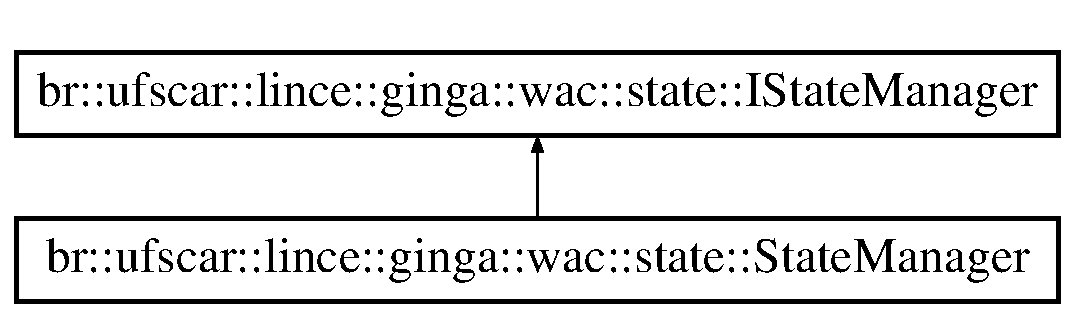
\includegraphics[height=2cm]{classbr_1_1ufscar_1_1lince_1_1ginga_1_1wac_1_1state_1_1IStateManager}
\end{center}
\end{figure}
\subsection*{Public Member Functions}
\begin{DoxyCompactItemize}
\item 
virtual void \hyperlink{classbr_1_1ufscar_1_1lince_1_1ginga_1_1wac_1_1state_1_1IStateManager_a739db8ceb6f56a110aa46bd272ea0956}{addStateProvider} (string id, \hyperlink{classbr_1_1ufscar_1_1lince_1_1ginga_1_1wac_1_1state_1_1IStateProvider}{IStateProvider} $\ast$stateProvider)=0
\begin{DoxyCompactList}\small\item\em Este método permite registrar uma instância capaz de informar parte do estado de uma apresentação NCL. \item\end{DoxyCompactList}\item 
virtual \hyperlink{classbr_1_1ufscar_1_1lince_1_1ginga_1_1wac_1_1state_1_1IPresentationState}{IPresentationState} $\ast$ \hyperlink{classbr_1_1ufscar_1_1lince_1_1ginga_1_1wac_1_1state_1_1IStateManager_a8fe894ac51f00b4d3633d93135678e0c}{getPresentationState} ()=0
\begin{DoxyCompactList}\small\item\em Este método gera um objeto que contém o estado da apresentação NCL ativa atual. \item\end{DoxyCompactList}\item 
virtual void \hyperlink{classbr_1_1ufscar_1_1lince_1_1ginga_1_1wac_1_1state_1_1IStateManager_a3e9493dcb1e1dbfd6171252fb2edca8d}{setContextProvider} (\hyperlink{classbr_1_1ufscar_1_1lince_1_1ginga_1_1wac_1_1state_1_1IContextProvider}{IContextProvider} $\ast$contextProvider)=0
\begin{DoxyCompactList}\small\item\em Este método permite registrar a instância responsável por fornecer o contexto da apresentação NCL. \item\end{DoxyCompactList}\item 
virtual \hyperlink{classbr_1_1ufscar_1_1lince_1_1ginga_1_1wac_1_1state_1_1IStateManager_afde1134f339b28a3a262f3df65857cc1}{$\sim$IStateManager} ()
\begin{DoxyCompactList}\small\item\em Destrutor Genérico. \item\end{DoxyCompactList}\end{DoxyCompactItemize}


\subsection{Detailed Description}
Está classe virtual é utilizada como interface para acessar os serviços providos pelo componente de \hyperlink{classbr_1_1ufscar_1_1lince_1_1ginga_1_1wac_1_1state_1_1StateManager}{StateManager}. 

\subsection{Constructor \& Destructor Documentation}
\hypertarget{classbr_1_1ufscar_1_1lince_1_1ginga_1_1wac_1_1state_1_1IStateManager_afde1134f339b28a3a262f3df65857cc1}{
\index{br::ufscar::lince::ginga::wac::state::IStateManager@{br::ufscar::lince::ginga::wac::state::IStateManager}!$\sim$IStateManager@{$\sim$IStateManager}}
\index{$\sim$IStateManager@{$\sim$IStateManager}!br::ufscar::lince::ginga::wac::state::IStateManager@{br::ufscar::lince::ginga::wac::state::IStateManager}}
\subsubsection[{$\sim$IStateManager}]{\setlength{\rightskip}{0pt plus 5cm}virtual br::ufscar::lince::ginga::wac::state::IStateManager::$\sim$IStateManager ()\hspace{0.3cm}{\ttfamily  \mbox{[}inline, virtual\mbox{]}}}}
\label{classbr_1_1ufscar_1_1lince_1_1ginga_1_1wac_1_1state_1_1IStateManager_afde1134f339b28a3a262f3df65857cc1}


Destrutor Genérico. 



\subsection{Member Function Documentation}
\hypertarget{classbr_1_1ufscar_1_1lince_1_1ginga_1_1wac_1_1state_1_1IStateManager_a739db8ceb6f56a110aa46bd272ea0956}{
\index{br::ufscar::lince::ginga::wac::state::IStateManager@{br::ufscar::lince::ginga::wac::state::IStateManager}!addStateProvider@{addStateProvider}}
\index{addStateProvider@{addStateProvider}!br::ufscar::lince::ginga::wac::state::IStateManager@{br::ufscar::lince::ginga::wac::state::IStateManager}}
\subsubsection[{addStateProvider}]{\setlength{\rightskip}{0pt plus 5cm}virtual void br::ufscar::lince::ginga::wac::state::IStateManager::addStateProvider (string {\em id}, \/  {\bf IStateProvider} $\ast$ {\em stateProvider})\hspace{0.3cm}{\ttfamily  \mbox{[}pure virtual\mbox{]}}}}
\label{classbr_1_1ufscar_1_1lince_1_1ginga_1_1wac_1_1state_1_1IStateManager_a739db8ceb6f56a110aa46bd272ea0956}


Este método permite registrar uma instância capaz de informar parte do estado de uma apresentação NCL. 


\begin{DoxyParams}{Parameters}
\item[{\em id}]Identificador do provedor de estados. \item[{\em stateProvider}]A instância do provedor de estados da aplicação \end{DoxyParams}


Implemented in \hyperlink{classbr_1_1ufscar_1_1lince_1_1ginga_1_1wac_1_1state_1_1StateManager_aa02a5c2cc3e5933a60225dc1b67e75e8}{br::ufscar::lince::ginga::wac::state::StateManager}.

\hypertarget{classbr_1_1ufscar_1_1lince_1_1ginga_1_1wac_1_1state_1_1IStateManager_a8fe894ac51f00b4d3633d93135678e0c}{
\index{br::ufscar::lince::ginga::wac::state::IStateManager@{br::ufscar::lince::ginga::wac::state::IStateManager}!getPresentationState@{getPresentationState}}
\index{getPresentationState@{getPresentationState}!br::ufscar::lince::ginga::wac::state::IStateManager@{br::ufscar::lince::ginga::wac::state::IStateManager}}
\subsubsection[{getPresentationState}]{\setlength{\rightskip}{0pt plus 5cm}virtual {\bf IPresentationState}$\ast$ br::ufscar::lince::ginga::wac::state::IStateManager::getPresentationState ()\hspace{0.3cm}{\ttfamily  \mbox{[}pure virtual\mbox{]}}}}
\label{classbr_1_1ufscar_1_1lince_1_1ginga_1_1wac_1_1state_1_1IStateManager_a8fe894ac51f00b4d3633d93135678e0c}


Este método gera um objeto que contém o estado da apresentação NCL ativa atual. 

\begin{DoxyReturn}{Returns}
Uma instância de \hyperlink{classbr_1_1ufscar_1_1lince_1_1ginga_1_1wac_1_1state_1_1IPresentationState}{IPresentationState} que contém o estado atual da apresentação NCL. 
\end{DoxyReturn}


Implemented in \hyperlink{classbr_1_1ufscar_1_1lince_1_1ginga_1_1wac_1_1state_1_1StateManager_affbdaf15d59f7df0aa182944818c3ad8}{br::ufscar::lince::ginga::wac::state::StateManager}.

\hypertarget{classbr_1_1ufscar_1_1lince_1_1ginga_1_1wac_1_1state_1_1IStateManager_a3e9493dcb1e1dbfd6171252fb2edca8d}{
\index{br::ufscar::lince::ginga::wac::state::IStateManager@{br::ufscar::lince::ginga::wac::state::IStateManager}!setContextProvider@{setContextProvider}}
\index{setContextProvider@{setContextProvider}!br::ufscar::lince::ginga::wac::state::IStateManager@{br::ufscar::lince::ginga::wac::state::IStateManager}}
\subsubsection[{setContextProvider}]{\setlength{\rightskip}{0pt plus 5cm}virtual void br::ufscar::lince::ginga::wac::state::IStateManager::setContextProvider ({\bf IContextProvider} $\ast$ {\em contextProvider})\hspace{0.3cm}{\ttfamily  \mbox{[}pure virtual\mbox{]}}}}
\label{classbr_1_1ufscar_1_1lince_1_1ginga_1_1wac_1_1state_1_1IStateManager_a3e9493dcb1e1dbfd6171252fb2edca8d}


Este método permite registrar a instância responsável por fornecer o contexto da apresentação NCL. 


\begin{DoxyParams}{Parameters}
\item[{\em contextProvider}]A instância que fornecerá o contexto da apresentação NCL. \end{DoxyParams}


Implemented in \hyperlink{classbr_1_1ufscar_1_1lince_1_1ginga_1_1wac_1_1state_1_1StateManager_a118df2766ab99574653b4f45d1ea75fd}{br::ufscar::lince::ginga::wac::state::StateManager}.



The documentation for this class was generated from the following file:\begin{DoxyCompactItemize}
\item 
include/\hyperlink{IStateManager_8h}{IStateManager.h}\end{DoxyCompactItemize}

\hypertarget{classbr_1_1ufscar_1_1lince_1_1ginga_1_1wac_1_1state_1_1IStateProvider}{
\section{br::ufscar::lince::ginga::wac::state::IStateProvider Class Reference}
\label{classbr_1_1ufscar_1_1lince_1_1ginga_1_1wac_1_1state_1_1IStateProvider}\index{br::ufscar::lince::ginga::wac::state::IStateProvider@{br::ufscar::lince::ginga::wac::state::IStateProvider}}
}


Interface utilizada para se obter o PlayerState das classes Players do módulo Formatter.  




{\ttfamily \#include $<$IStateProvider.h$>$}

\subsection*{Public Member Functions}
\begin{DoxyCompactItemize}
\item 
virtual PlayerState $\ast$ \hyperlink{classbr_1_1ufscar_1_1lince_1_1ginga_1_1wac_1_1state_1_1IStateProvider_a9616b84638f876ff749ffd8c76162f78}{getPlayerState} ()=0
\begin{DoxyCompactList}\small\item\em Retorna o estado atual do player. \item\end{DoxyCompactList}\item 
virtual \hyperlink{classbr_1_1ufscar_1_1lince_1_1ginga_1_1wac_1_1state_1_1IStateProvider_a5a3e4a2209741be59347f6a0d7ba6732}{$\sim$IStateProvider} ()
\end{DoxyCompactItemize}


\subsection{Detailed Description}
Interface utilizada para se obter o PlayerState das classes Players do módulo Formatter. Esta interface deve ser implementada pelas classes PlayerAdapter do módulo Formatter do Ginga para que seja possível se obter os estados correntes de cada player em execução. 

\subsection{Constructor \& Destructor Documentation}
\hypertarget{classbr_1_1ufscar_1_1lince_1_1ginga_1_1wac_1_1state_1_1IStateProvider_a5a3e4a2209741be59347f6a0d7ba6732}{
\index{br::ufscar::lince::ginga::wac::state::IStateProvider@{br::ufscar::lince::ginga::wac::state::IStateProvider}!$\sim$IStateProvider@{$\sim$IStateProvider}}
\index{$\sim$IStateProvider@{$\sim$IStateProvider}!br::ufscar::lince::ginga::wac::state::IStateProvider@{br::ufscar::lince::ginga::wac::state::IStateProvider}}
\subsubsection[{$\sim$IStateProvider}]{\setlength{\rightskip}{0pt plus 5cm}virtual br::ufscar::lince::ginga::wac::state::IStateProvider::$\sim$IStateProvider ()\hspace{0.3cm}{\ttfamily  \mbox{[}inline, virtual\mbox{]}}}}
\label{classbr_1_1ufscar_1_1lince_1_1ginga_1_1wac_1_1state_1_1IStateProvider_a5a3e4a2209741be59347f6a0d7ba6732}


\subsection{Member Function Documentation}
\hypertarget{classbr_1_1ufscar_1_1lince_1_1ginga_1_1wac_1_1state_1_1IStateProvider_a9616b84638f876ff749ffd8c76162f78}{
\index{br::ufscar::lince::ginga::wac::state::IStateProvider@{br::ufscar::lince::ginga::wac::state::IStateProvider}!getPlayerState@{getPlayerState}}
\index{getPlayerState@{getPlayerState}!br::ufscar::lince::ginga::wac::state::IStateProvider@{br::ufscar::lince::ginga::wac::state::IStateProvider}}
\subsubsection[{getPlayerState}]{\setlength{\rightskip}{0pt plus 5cm}virtual PlayerState$\ast$ br::ufscar::lince::ginga::wac::state::IStateProvider::getPlayerState ()\hspace{0.3cm}{\ttfamily  \mbox{[}pure virtual\mbox{]}}}}
\label{classbr_1_1ufscar_1_1lince_1_1ginga_1_1wac_1_1state_1_1IStateProvider_a9616b84638f876ff749ffd8c76162f78}


Retorna o estado atual do player. 

Instância de PlayerState que contém as informações do estado atual do player. 

The documentation for this class was generated from the following file:\begin{DoxyCompactItemize}
\item 
include/\hyperlink{IStateProvider_8h}{IStateProvider.h}\end{DoxyCompactItemize}

\hypertarget{classbr_1_1ufscar_1_1lince_1_1ginga_1_1wac_1_1state_1_1PresentationState}{
\section{br::ufscar::lince::ginga::wac::state::PresentationState Class Reference}
\label{classbr_1_1ufscar_1_1lince_1_1ginga_1_1wac_1_1state_1_1PresentationState}\index{br::ufscar::lince::ginga::wac::state::PresentationState@{br::ufscar::lince::ginga::wac::state::PresentationState}}
}


Representa o estado da apresentação como um todo em um dado momento.  




{\ttfamily \#include $<$PresentationState.h$>$}

Inheritance diagram for br::ufscar::lince::ginga::wac::state::PresentationState:\begin{figure}[H]
\begin{center}
\leavevmode
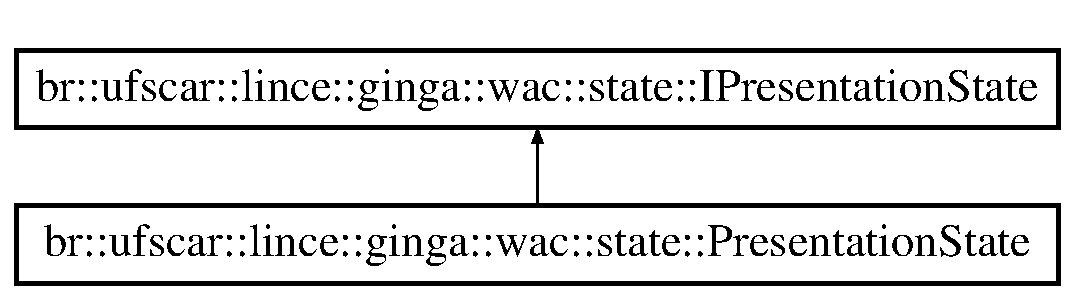
\includegraphics[height=2cm]{classbr_1_1ufscar_1_1lince_1_1ginga_1_1wac_1_1state_1_1PresentationState}
\end{center}
\end{figure}
\subsection*{Public Member Functions}
\begin{DoxyCompactItemize}
\item 
\hyperlink{classbr_1_1ufscar_1_1lince_1_1ginga_1_1wac_1_1state_1_1PresentationState_aa48f61ac6a0cf382182bd6fb4f548b87}{PresentationState} ()
\begin{DoxyCompactList}\small\item\em Constrói uma instância de \hyperlink{classbr_1_1ufscar_1_1lince_1_1ginga_1_1wac_1_1state_1_1PresentationState}{PresentationState}. \item\end{DoxyCompactList}\item 
\hyperlink{classbr_1_1ufscar_1_1lince_1_1ginga_1_1wac_1_1state_1_1PresentationState_a324581a9a822f53cf7365321ae35f2ec}{$\sim$PresentationState} ()
\begin{DoxyCompactList}\small\item\em Destrói a instância de \hyperlink{classbr_1_1ufscar_1_1lince_1_1ginga_1_1wac_1_1state_1_1PresentationState}{PresentationState}. \item\end{DoxyCompactList}\item 
void \hyperlink{classbr_1_1ufscar_1_1lince_1_1ginga_1_1wac_1_1state_1_1PresentationState_a02bf97b60acc4e5ba168961d8e695195}{setStateMap} (map$<$ string, \hyperlink{classbr_1_1ufscar_1_1lince_1_1ginga_1_1wac_1_1state_1_1IElementaryState}{IElementaryState} $\ast$ $>$ $\ast$nStateMap, map$<$ string, string $>$ $\ast$nDescMap, map$<$ string, string $>$ $\ast$nContextMap)
\begin{DoxyCompactList}\small\item\em Seta os mapas que contém os estados dos players da apresentação. \item\end{DoxyCompactList}\item 
void \hyperlink{classbr_1_1ufscar_1_1lince_1_1ginga_1_1wac_1_1state_1_1PresentationState_aadc7632e1bff7b0c2680a5193679e1d9}{setDcoumentName} (string name)
\begin{DoxyCompactList}\small\item\em Seta o nome do documento NCL. \item\end{DoxyCompactList}\item 
void \hyperlink{classbr_1_1ufscar_1_1lince_1_1ginga_1_1wac_1_1state_1_1PresentationState_a127842284622579c23ec1d6ce974fe8f}{setPrivateBaseName} (string name)
\begin{DoxyCompactList}\small\item\em Seta o nome da base privada. \item\end{DoxyCompactList}\item 
virtual vector$<$ string $>$ $\ast$ \hyperlink{classbr_1_1ufscar_1_1lince_1_1ginga_1_1wac_1_1state_1_1PresentationState_a82bc0879c2e2d6c6eb48ffaeee043bac}{getPlayersNames} ()
\begin{DoxyCompactList}\small\item\em Retorna o nome de todos os players da apresentação atual. \item\end{DoxyCompactList}\item 
virtual \hyperlink{classbr_1_1ufscar_1_1lince_1_1ginga_1_1wac_1_1state_1_1IElementaryState}{IElementaryState} $\ast$ \hyperlink{classbr_1_1ufscar_1_1lince_1_1ginga_1_1wac_1_1state_1_1PresentationState_a460f75f353ea3508dacdbd2a29bd537e}{getElementaryState} (string name)
\begin{DoxyCompactList}\small\item\em Retorna o estado de um determinado Player. \item\end{DoxyCompactList}\item 
virtual string \hyperlink{classbr_1_1ufscar_1_1lince_1_1ginga_1_1wac_1_1state_1_1PresentationState_a5f3306aca36ba9aac7c43d27f6f29ad9}{getMediaDescriptor} (string name)
\begin{DoxyCompactList}\small\item\em Retorna o Descritor associado ao nó de mídia de um player. \item\end{DoxyCompactList}\item 
virtual string \hyperlink{classbr_1_1ufscar_1_1lince_1_1ginga_1_1wac_1_1state_1_1PresentationState_af4149387468f9a7180c036f4fdce03bd}{getPresentationName} ()
\begin{DoxyCompactList}\small\item\em Retorna o nome completo da apresentação. \item\end{DoxyCompactList}\item 
virtual string \hyperlink{classbr_1_1ufscar_1_1lince_1_1ginga_1_1wac_1_1state_1_1PresentationState_a90a8797bdaffaed86c5a686652fea889}{getDocumentName} ()
\begin{DoxyCompactList}\small\item\em Retorna o nome do documento NCL. \item\end{DoxyCompactList}\item 
virtual string \hyperlink{classbr_1_1ufscar_1_1lince_1_1ginga_1_1wac_1_1state_1_1PresentationState_a5b280537bd03a744eb41807859f01413}{getPrivateBaseName} ()
\begin{DoxyCompactList}\small\item\em Retorna o nome da base privada. \item\end{DoxyCompactList}\item 
virtual string \hyperlink{classbr_1_1ufscar_1_1lince_1_1ginga_1_1wac_1_1state_1_1PresentationState_a00ec06809774af254532488cc1559c15}{toString} ()
\begin{DoxyCompactList}\small\item\em Retorna uma string contento o resumo das principais informações relativas ao estado da apresentação presentados pelo objeto. \item\end{DoxyCompactList}\item 
virtual vector$<$ string $>$ $\ast$ \hyperlink{classbr_1_1ufscar_1_1lince_1_1ginga_1_1wac_1_1state_1_1PresentationState_ab5f9e22342f390d01e54ca51f8a85609}{getContextPropertyNames} ()
\begin{DoxyCompactList}\small\item\em Este método retorna todos os nomes das propriedades relativas ao contexto da apresentação. \item\end{DoxyCompactList}\item 
virtual string \hyperlink{classbr_1_1ufscar_1_1lince_1_1ginga_1_1wac_1_1state_1_1PresentationState_a2931ba17e6dcd1352382fee289352f4b}{getContextPropertyValue} (string attributeId)
\begin{DoxyCompactList}\small\item\em Este método retorna o valor de uma determinada propriedade do contexto da apresentação através de uma string. \item\end{DoxyCompactList}\end{DoxyCompactItemize}


\subsection{Detailed Description}
Representa o estado da apresentação como um todo em um dado momento. Esta classe agrupa o estado de todos os players de uma apresentação NCL além de outras informações mais gerais da apresentação, representado o estado de uma apresentação NCL em um dado momento. 

\subsection{Constructor \& Destructor Documentation}
\hypertarget{classbr_1_1ufscar_1_1lince_1_1ginga_1_1wac_1_1state_1_1PresentationState_aa48f61ac6a0cf382182bd6fb4f548b87}{
\index{br::ufscar::lince::ginga::wac::state::PresentationState@{br::ufscar::lince::ginga::wac::state::PresentationState}!PresentationState@{PresentationState}}
\index{PresentationState@{PresentationState}!br::ufscar::lince::ginga::wac::state::PresentationState@{br::ufscar::lince::ginga::wac::state::PresentationState}}
\subsubsection[{PresentationState}]{\setlength{\rightskip}{0pt plus 5cm}br::ufscar::lince::ginga::wac::state::PresentationState::PresentationState ()}}
\label{classbr_1_1ufscar_1_1lince_1_1ginga_1_1wac_1_1state_1_1PresentationState_aa48f61ac6a0cf382182bd6fb4f548b87}


Constrói uma instância de \hyperlink{classbr_1_1ufscar_1_1lince_1_1ginga_1_1wac_1_1state_1_1PresentationState}{PresentationState}. 

\hypertarget{classbr_1_1ufscar_1_1lince_1_1ginga_1_1wac_1_1state_1_1PresentationState_a324581a9a822f53cf7365321ae35f2ec}{
\index{br::ufscar::lince::ginga::wac::state::PresentationState@{br::ufscar::lince::ginga::wac::state::PresentationState}!$\sim$PresentationState@{$\sim$PresentationState}}
\index{$\sim$PresentationState@{$\sim$PresentationState}!br::ufscar::lince::ginga::wac::state::PresentationState@{br::ufscar::lince::ginga::wac::state::PresentationState}}
\subsubsection[{$\sim$PresentationState}]{\setlength{\rightskip}{0pt plus 5cm}br::ufscar::lince::ginga::wac::state::PresentationState::$\sim$PresentationState ()}}
\label{classbr_1_1ufscar_1_1lince_1_1ginga_1_1wac_1_1state_1_1PresentationState_a324581a9a822f53cf7365321ae35f2ec}


Destrói a instância de \hyperlink{classbr_1_1ufscar_1_1lince_1_1ginga_1_1wac_1_1state_1_1PresentationState}{PresentationState}. 



\subsection{Member Function Documentation}
\hypertarget{classbr_1_1ufscar_1_1lince_1_1ginga_1_1wac_1_1state_1_1PresentationState_ab5f9e22342f390d01e54ca51f8a85609}{
\index{br::ufscar::lince::ginga::wac::state::PresentationState@{br::ufscar::lince::ginga::wac::state::PresentationState}!getContextPropertyNames@{getContextPropertyNames}}
\index{getContextPropertyNames@{getContextPropertyNames}!br::ufscar::lince::ginga::wac::state::PresentationState@{br::ufscar::lince::ginga::wac::state::PresentationState}}
\subsubsection[{getContextPropertyNames}]{\setlength{\rightskip}{0pt plus 5cm}virtual vector$<$string$>$$\ast$ br::ufscar::lince::ginga::wac::state::PresentationState::getContextPropertyNames ()\hspace{0.3cm}{\ttfamily  \mbox{[}virtual\mbox{]}}}}
\label{classbr_1_1ufscar_1_1lince_1_1ginga_1_1wac_1_1state_1_1PresentationState_ab5f9e22342f390d01e54ca51f8a85609}


Este método retorna todos os nomes das propriedades relativas ao contexto da apresentação. 


\begin{DoxyParams}{Parameters}
\item[{\em Um}]vetor contento o nome das propriedades relativas ao contexto. \end{DoxyParams}


Implements \hyperlink{classbr_1_1ufscar_1_1lince_1_1ginga_1_1wac_1_1state_1_1IPresentationState_a3ec5c1d54f31461e1a3e81a54fefaa87}{br::ufscar::lince::ginga::wac::state::IPresentationState}.

\hypertarget{classbr_1_1ufscar_1_1lince_1_1ginga_1_1wac_1_1state_1_1PresentationState_a2931ba17e6dcd1352382fee289352f4b}{
\index{br::ufscar::lince::ginga::wac::state::PresentationState@{br::ufscar::lince::ginga::wac::state::PresentationState}!getContextPropertyValue@{getContextPropertyValue}}
\index{getContextPropertyValue@{getContextPropertyValue}!br::ufscar::lince::ginga::wac::state::PresentationState@{br::ufscar::lince::ginga::wac::state::PresentationState}}
\subsubsection[{getContextPropertyValue}]{\setlength{\rightskip}{0pt plus 5cm}virtual string br::ufscar::lince::ginga::wac::state::PresentationState::getContextPropertyValue (string {\em attributeId})\hspace{0.3cm}{\ttfamily  \mbox{[}virtual\mbox{]}}}}
\label{classbr_1_1ufscar_1_1lince_1_1ginga_1_1wac_1_1state_1_1PresentationState_a2931ba17e6dcd1352382fee289352f4b}


Este método retorna o valor de uma determinada propriedade do contexto da apresentação através de uma string. 


\begin{DoxyParams}{Parameters}
\item[{\em attributeId}]O identificador da propriedade do contexto. \end{DoxyParams}
\begin{DoxyReturn}{Returns}
O valor da propriedade representada através de uma string 
\end{DoxyReturn}


Implements \hyperlink{classbr_1_1ufscar_1_1lince_1_1ginga_1_1wac_1_1state_1_1IPresentationState_a3d16c8c6c2c90ef84313414072d953cf}{br::ufscar::lince::ginga::wac::state::IPresentationState}.

\hypertarget{classbr_1_1ufscar_1_1lince_1_1ginga_1_1wac_1_1state_1_1PresentationState_a90a8797bdaffaed86c5a686652fea889}{
\index{br::ufscar::lince::ginga::wac::state::PresentationState@{br::ufscar::lince::ginga::wac::state::PresentationState}!getDocumentName@{getDocumentName}}
\index{getDocumentName@{getDocumentName}!br::ufscar::lince::ginga::wac::state::PresentationState@{br::ufscar::lince::ginga::wac::state::PresentationState}}
\subsubsection[{getDocumentName}]{\setlength{\rightskip}{0pt plus 5cm}virtual string br::ufscar::lince::ginga::wac::state::PresentationState::getDocumentName ()\hspace{0.3cm}{\ttfamily  \mbox{[}virtual\mbox{]}}}}
\label{classbr_1_1ufscar_1_1lince_1_1ginga_1_1wac_1_1state_1_1PresentationState_a90a8797bdaffaed86c5a686652fea889}


Retorna o nome do documento NCL. 

\begin{DoxyReturn}{Returns}
String contendo o nome do documento NCL. 
\end{DoxyReturn}


Implements \hyperlink{classbr_1_1ufscar_1_1lince_1_1ginga_1_1wac_1_1state_1_1IPresentationState_a20c06c68a1db0160932abf7d6aa4967c}{br::ufscar::lince::ginga::wac::state::IPresentationState}.

\hypertarget{classbr_1_1ufscar_1_1lince_1_1ginga_1_1wac_1_1state_1_1PresentationState_a460f75f353ea3508dacdbd2a29bd537e}{
\index{br::ufscar::lince::ginga::wac::state::PresentationState@{br::ufscar::lince::ginga::wac::state::PresentationState}!getElementaryState@{getElementaryState}}
\index{getElementaryState@{getElementaryState}!br::ufscar::lince::ginga::wac::state::PresentationState@{br::ufscar::lince::ginga::wac::state::PresentationState}}
\subsubsection[{getElementaryState}]{\setlength{\rightskip}{0pt plus 5cm}virtual {\bf IElementaryState}$\ast$ br::ufscar::lince::ginga::wac::state::PresentationState::getElementaryState (string {\em name})\hspace{0.3cm}{\ttfamily  \mbox{[}virtual\mbox{]}}}}
\label{classbr_1_1ufscar_1_1lince_1_1ginga_1_1wac_1_1state_1_1PresentationState_a460f75f353ea3508dacdbd2a29bd537e}


Retorna o estado de um determinado Player. 


\begin{DoxyParams}{Parameters}
\item[{\em name}]Nome do player o qual se deseja obter o estado. \end{DoxyParams}
\begin{DoxyReturn}{Returns}
Instância de PlayerStateWac com o estado atual do player. 
\end{DoxyReturn}


Implements \hyperlink{classbr_1_1ufscar_1_1lince_1_1ginga_1_1wac_1_1state_1_1IPresentationState_a42e36ac35404e13df2b3df4f2da614a1}{br::ufscar::lince::ginga::wac::state::IPresentationState}.

\hypertarget{classbr_1_1ufscar_1_1lince_1_1ginga_1_1wac_1_1state_1_1PresentationState_a5f3306aca36ba9aac7c43d27f6f29ad9}{
\index{br::ufscar::lince::ginga::wac::state::PresentationState@{br::ufscar::lince::ginga::wac::state::PresentationState}!getMediaDescriptor@{getMediaDescriptor}}
\index{getMediaDescriptor@{getMediaDescriptor}!br::ufscar::lince::ginga::wac::state::PresentationState@{br::ufscar::lince::ginga::wac::state::PresentationState}}
\subsubsection[{getMediaDescriptor}]{\setlength{\rightskip}{0pt plus 5cm}virtual string br::ufscar::lince::ginga::wac::state::PresentationState::getMediaDescriptor (string {\em name})\hspace{0.3cm}{\ttfamily  \mbox{[}virtual\mbox{]}}}}
\label{classbr_1_1ufscar_1_1lince_1_1ginga_1_1wac_1_1state_1_1PresentationState_a5f3306aca36ba9aac7c43d27f6f29ad9}


Retorna o Descritor associado ao nó de mídia de um player. 


\begin{DoxyParams}{Parameters}
\item[{\em Nome}]do Player relacionado ao nó de mídia. \end{DoxyParams}
\begin{DoxyReturn}{Returns}
Nome do descritor associado ao nó de mídia. 
\end{DoxyReturn}


Implements \hyperlink{classbr_1_1ufscar_1_1lince_1_1ginga_1_1wac_1_1state_1_1IPresentationState_a4a8d2526ea16319ea1efc19928ffe028}{br::ufscar::lince::ginga::wac::state::IPresentationState}.

\hypertarget{classbr_1_1ufscar_1_1lince_1_1ginga_1_1wac_1_1state_1_1PresentationState_a82bc0879c2e2d6c6eb48ffaeee043bac}{
\index{br::ufscar::lince::ginga::wac::state::PresentationState@{br::ufscar::lince::ginga::wac::state::PresentationState}!getPlayersNames@{getPlayersNames}}
\index{getPlayersNames@{getPlayersNames}!br::ufscar::lince::ginga::wac::state::PresentationState@{br::ufscar::lince::ginga::wac::state::PresentationState}}
\subsubsection[{getPlayersNames}]{\setlength{\rightskip}{0pt plus 5cm}virtual vector$<$string$>$$\ast$ br::ufscar::lince::ginga::wac::state::PresentationState::getPlayersNames ()\hspace{0.3cm}{\ttfamily  \mbox{[}virtual\mbox{]}}}}
\label{classbr_1_1ufscar_1_1lince_1_1ginga_1_1wac_1_1state_1_1PresentationState_a82bc0879c2e2d6c6eb48ffaeee043bac}


Retorna o nome de todos os players da apresentação atual. 

\begin{DoxyReturn}{Returns}
Instância de vector contendo todos os nomes dos players da apresentação atual. 
\end{DoxyReturn}


Implements \hyperlink{classbr_1_1ufscar_1_1lince_1_1ginga_1_1wac_1_1state_1_1IPresentationState_ac3ba6e82191af041b1bc4320ddaf0ca5}{br::ufscar::lince::ginga::wac::state::IPresentationState}.

\hypertarget{classbr_1_1ufscar_1_1lince_1_1ginga_1_1wac_1_1state_1_1PresentationState_af4149387468f9a7180c036f4fdce03bd}{
\index{br::ufscar::lince::ginga::wac::state::PresentationState@{br::ufscar::lince::ginga::wac::state::PresentationState}!getPresentationName@{getPresentationName}}
\index{getPresentationName@{getPresentationName}!br::ufscar::lince::ginga::wac::state::PresentationState@{br::ufscar::lince::ginga::wac::state::PresentationState}}
\subsubsection[{getPresentationName}]{\setlength{\rightskip}{0pt plus 5cm}virtual string br::ufscar::lince::ginga::wac::state::PresentationState::getPresentationName ()\hspace{0.3cm}{\ttfamily  \mbox{[}virtual\mbox{]}}}}
\label{classbr_1_1ufscar_1_1lince_1_1ginga_1_1wac_1_1state_1_1PresentationState_af4149387468f9a7180c036f4fdce03bd}


Retorna o nome completo da apresentação. 

\begin{DoxyReturn}{Returns}
String contendo o nome completo da apresentação; 
\end{DoxyReturn}


Implements \hyperlink{classbr_1_1ufscar_1_1lince_1_1ginga_1_1wac_1_1state_1_1IPresentationState_a939e322cd15e49680f227bfc6b9ded9d}{br::ufscar::lince::ginga::wac::state::IPresentationState}.

\hypertarget{classbr_1_1ufscar_1_1lince_1_1ginga_1_1wac_1_1state_1_1PresentationState_a5b280537bd03a744eb41807859f01413}{
\index{br::ufscar::lince::ginga::wac::state::PresentationState@{br::ufscar::lince::ginga::wac::state::PresentationState}!getPrivateBaseName@{getPrivateBaseName}}
\index{getPrivateBaseName@{getPrivateBaseName}!br::ufscar::lince::ginga::wac::state::PresentationState@{br::ufscar::lince::ginga::wac::state::PresentationState}}
\subsubsection[{getPrivateBaseName}]{\setlength{\rightskip}{0pt plus 5cm}virtual string br::ufscar::lince::ginga::wac::state::PresentationState::getPrivateBaseName ()\hspace{0.3cm}{\ttfamily  \mbox{[}virtual\mbox{]}}}}
\label{classbr_1_1ufscar_1_1lince_1_1ginga_1_1wac_1_1state_1_1PresentationState_a5b280537bd03a744eb41807859f01413}


Retorna o nome da base privada. 

\begin{DoxyReturn}{Returns}
String contendo o nome da base privada. 
\end{DoxyReturn}


Implements \hyperlink{classbr_1_1ufscar_1_1lince_1_1ginga_1_1wac_1_1state_1_1IPresentationState_a53e509fcb89622fa57b299526f96f728}{br::ufscar::lince::ginga::wac::state::IPresentationState}.

\hypertarget{classbr_1_1ufscar_1_1lince_1_1ginga_1_1wac_1_1state_1_1PresentationState_aadc7632e1bff7b0c2680a5193679e1d9}{
\index{br::ufscar::lince::ginga::wac::state::PresentationState@{br::ufscar::lince::ginga::wac::state::PresentationState}!setDcoumentName@{setDcoumentName}}
\index{setDcoumentName@{setDcoumentName}!br::ufscar::lince::ginga::wac::state::PresentationState@{br::ufscar::lince::ginga::wac::state::PresentationState}}
\subsubsection[{setDcoumentName}]{\setlength{\rightskip}{0pt plus 5cm}void br::ufscar::lince::ginga::wac::state::PresentationState::setDcoumentName (string {\em name})}}
\label{classbr_1_1ufscar_1_1lince_1_1ginga_1_1wac_1_1state_1_1PresentationState_aadc7632e1bff7b0c2680a5193679e1d9}


Seta o nome do documento NCL. 


\begin{DoxyParams}{Parameters}
\item[{\em name}]Nome do documento NCL. \end{DoxyParams}
\hypertarget{classbr_1_1ufscar_1_1lince_1_1ginga_1_1wac_1_1state_1_1PresentationState_a127842284622579c23ec1d6ce974fe8f}{
\index{br::ufscar::lince::ginga::wac::state::PresentationState@{br::ufscar::lince::ginga::wac::state::PresentationState}!setPrivateBaseName@{setPrivateBaseName}}
\index{setPrivateBaseName@{setPrivateBaseName}!br::ufscar::lince::ginga::wac::state::PresentationState@{br::ufscar::lince::ginga::wac::state::PresentationState}}
\subsubsection[{setPrivateBaseName}]{\setlength{\rightskip}{0pt plus 5cm}void br::ufscar::lince::ginga::wac::state::PresentationState::setPrivateBaseName (string {\em name})}}
\label{classbr_1_1ufscar_1_1lince_1_1ginga_1_1wac_1_1state_1_1PresentationState_a127842284622579c23ec1d6ce974fe8f}


Seta o nome da base privada. 


\begin{DoxyParams}{Parameters}
\item[{\em name}]Nome da base privada. \end{DoxyParams}
\hypertarget{classbr_1_1ufscar_1_1lince_1_1ginga_1_1wac_1_1state_1_1PresentationState_a02bf97b60acc4e5ba168961d8e695195}{
\index{br::ufscar::lince::ginga::wac::state::PresentationState@{br::ufscar::lince::ginga::wac::state::PresentationState}!setStateMap@{setStateMap}}
\index{setStateMap@{setStateMap}!br::ufscar::lince::ginga::wac::state::PresentationState@{br::ufscar::lince::ginga::wac::state::PresentationState}}
\subsubsection[{setStateMap}]{\setlength{\rightskip}{0pt plus 5cm}void br::ufscar::lince::ginga::wac::state::PresentationState::setStateMap (map$<$ string, {\bf IElementaryState} $\ast$ $>$ $\ast$ {\em nStateMap}, \/  map$<$ string, string $>$ $\ast$ {\em nDescMap}, \/  map$<$ string, string $>$ $\ast$ {\em nContextMap})}}
\label{classbr_1_1ufscar_1_1lince_1_1ginga_1_1wac_1_1state_1_1PresentationState_a02bf97b60acc4e5ba168961d8e695195}


Seta os mapas que contém os estados dos players da apresentação. 


\begin{DoxyParams}{Parameters}
\item[{\em nStateMap}]Mapa que relaciona os nomes dos players com seus estados. \item[{\em nDescMap}]Mapa que relaciona os nomes dos players com seus descritores. \end{DoxyParams}
\hypertarget{classbr_1_1ufscar_1_1lince_1_1ginga_1_1wac_1_1state_1_1PresentationState_a00ec06809774af254532488cc1559c15}{
\index{br::ufscar::lince::ginga::wac::state::PresentationState@{br::ufscar::lince::ginga::wac::state::PresentationState}!toString@{toString}}
\index{toString@{toString}!br::ufscar::lince::ginga::wac::state::PresentationState@{br::ufscar::lince::ginga::wac::state::PresentationState}}
\subsubsection[{toString}]{\setlength{\rightskip}{0pt plus 5cm}virtual string br::ufscar::lince::ginga::wac::state::PresentationState::toString ()\hspace{0.3cm}{\ttfamily  \mbox{[}virtual\mbox{]}}}}
\label{classbr_1_1ufscar_1_1lince_1_1ginga_1_1wac_1_1state_1_1PresentationState_a00ec06809774af254532488cc1559c15}


Retorna uma string contento o resumo das principais informações relativas ao estado da apresentação presentados pelo objeto. 

\begin{DoxyReturn}{Returns}
String com o resumo do estado da apresentaçaõ. 
\end{DoxyReturn}


Implements \hyperlink{classbr_1_1ufscar_1_1lince_1_1ginga_1_1wac_1_1state_1_1IPresentationState_a148a58eee3e6f96ae226f8360696d944}{br::ufscar::lince::ginga::wac::state::IPresentationState}.



The documentation for this class was generated from the following file:\begin{DoxyCompactItemize}
\item 
include/\hyperlink{PresentationState_8h}{PresentationState.h}\end{DoxyCompactItemize}

\hypertarget{classbr_1_1ufscar_1_1lince_1_1ginga_1_1wac_1_1state_1_1StateManager}{
\section{br::ufscar::lince::ginga::wac::state::StateManager Class Reference}
\label{classbr_1_1ufscar_1_1lince_1_1ginga_1_1wac_1_1state_1_1StateManager}\index{br::ufscar::lince::ginga::wac::state::StateManager@{br::ufscar::lince::ginga::wac::state::StateManager}}
}
\subsection*{Public Member Functions}
\begin{DoxyCompactItemize}
\item 
void \hyperlink{classbr_1_1ufscar_1_1lince_1_1ginga_1_1wac_1_1state_1_1StateManager_ab0b8ca8a349b9fbda4c9960fd72345df}{addPlayerAdapter} (string id, \hyperlink{classbr_1_1ufscar_1_1lince_1_1ginga_1_1wac_1_1state_1_1IPlayerWac}{IPlayerWac} $\ast$playerAd)
\begin{DoxyCompactList}\small\item\em Adiciona um player a lista de players monitorados pela \hyperlink{classbr_1_1ufscar_1_1lince_1_1ginga_1_1wac_1_1state_1_1StateManager}{StateManager}. \item\end{DoxyCompactList}\item 
\hyperlink{classbr_1_1ufscar_1_1lince_1_1ginga_1_1wac_1_1state_1_1PresentationState}{PresentationState} $\ast$ \hyperlink{classbr_1_1ufscar_1_1lince_1_1ginga_1_1wac_1_1state_1_1StateManager_ab7c82f257bf2515985a54e65bf546da5}{getPresentationState} ()
\begin{DoxyCompactList}\small\item\em Retorna o estado da apresentação no atual momento. \item\end{DoxyCompactList}\end{DoxyCompactItemize}
\subsection*{Static Public Member Functions}
\begin{DoxyCompactItemize}
\item 
static \hyperlink{classbr_1_1ufscar_1_1lince_1_1ginga_1_1wac_1_1state_1_1StateManager}{StateManager} $\ast$ \hyperlink{classbr_1_1ufscar_1_1lince_1_1ginga_1_1wac_1_1state_1_1StateManager_a7875cddb02bd5dfa72539234438b3a7e}{getInstance} ()
\begin{DoxyCompactList}\small\item\em Permite obter acesso a instância única de \hyperlink{classbr_1_1ufscar_1_1lince_1_1ginga_1_1wac_1_1state_1_1StateManager}{StateManager}. \item\end{DoxyCompactList}\end{DoxyCompactItemize}


\subsection{Member Function Documentation}
\hypertarget{classbr_1_1ufscar_1_1lince_1_1ginga_1_1wac_1_1state_1_1StateManager_ab0b8ca8a349b9fbda4c9960fd72345df}{
\index{br::ufscar::lince::ginga::wac::state::StateManager@{br::ufscar::lince::ginga::wac::state::StateManager}!addPlayerAdapter@{addPlayerAdapter}}
\index{addPlayerAdapter@{addPlayerAdapter}!br::ufscar::lince::ginga::wac::state::StateManager@{br::ufscar::lince::ginga::wac::state::StateManager}}
\subsubsection[{addPlayerAdapter}]{\setlength{\rightskip}{0pt plus 5cm}void br::ufscar::lince::ginga::wac::state::StateManager::addPlayerAdapter (string {\em id}, \/  {\bf IPlayerWac} $\ast$ {\em playerAd})}}
\label{classbr_1_1ufscar_1_1lince_1_1ginga_1_1wac_1_1state_1_1StateManager_ab0b8ca8a349b9fbda4c9960fd72345df}


Adiciona um player a lista de players monitorados pela \hyperlink{classbr_1_1ufscar_1_1lince_1_1ginga_1_1wac_1_1state_1_1StateManager}{StateManager}. 
\begin{DoxyParams}{Parameters}
\item[{\em id}]Identificador do Player dentro da Maquina de Apresentação NCL. \item[{\em playerAd}]Instância de PlayerAdapter que será monitorado por \hyperlink{classbr_1_1ufscar_1_1lince_1_1ginga_1_1wac_1_1state_1_1StateManager}{StateManager}. \end{DoxyParams}
\hypertarget{classbr_1_1ufscar_1_1lince_1_1ginga_1_1wac_1_1state_1_1StateManager_a7875cddb02bd5dfa72539234438b3a7e}{
\index{br::ufscar::lince::ginga::wac::state::StateManager@{br::ufscar::lince::ginga::wac::state::StateManager}!getInstance@{getInstance}}
\index{getInstance@{getInstance}!br::ufscar::lince::ginga::wac::state::StateManager@{br::ufscar::lince::ginga::wac::state::StateManager}}
\subsubsection[{getInstance}]{\setlength{\rightskip}{0pt plus 5cm}static {\bf StateManager}$\ast$ br::ufscar::lince::ginga::wac::state::StateManager::getInstance ()\hspace{0.3cm}{\ttfamily  \mbox{[}static\mbox{]}}}}
\label{classbr_1_1ufscar_1_1lince_1_1ginga_1_1wac_1_1state_1_1StateManager_a7875cddb02bd5dfa72539234438b3a7e}


Permite obter acesso a instância única de \hyperlink{classbr_1_1ufscar_1_1lince_1_1ginga_1_1wac_1_1state_1_1StateManager}{StateManager}. \begin{DoxyReturn}{Returns}
Instância única de \hyperlink{classbr_1_1ufscar_1_1lince_1_1ginga_1_1wac_1_1state_1_1StateManager}{StateManager}. 
\end{DoxyReturn}
\hypertarget{classbr_1_1ufscar_1_1lince_1_1ginga_1_1wac_1_1state_1_1StateManager_ab7c82f257bf2515985a54e65bf546da5}{
\index{br::ufscar::lince::ginga::wac::state::StateManager@{br::ufscar::lince::ginga::wac::state::StateManager}!getPresentationState@{getPresentationState}}
\index{getPresentationState@{getPresentationState}!br::ufscar::lince::ginga::wac::state::StateManager@{br::ufscar::lince::ginga::wac::state::StateManager}}
\subsubsection[{getPresentationState}]{\setlength{\rightskip}{0pt plus 5cm}{\bf PresentationState}$\ast$ br::ufscar::lince::ginga::wac::state::StateManager::getPresentationState ()}}
\label{classbr_1_1ufscar_1_1lince_1_1ginga_1_1wac_1_1state_1_1StateManager_ab7c82f257bf2515985a54e65bf546da5}


Retorna o estado da apresentação no atual momento. \begin{DoxyReturn}{Returns}
instância de \hyperlink{classbr_1_1ufscar_1_1lince_1_1ginga_1_1wac_1_1state_1_1PresentationState}{PresentationState} contento o estado atual da apresentação. 
\end{DoxyReturn}


The documentation for this class was generated from the following file:\begin{DoxyCompactItemize}
\item 
\hyperlink{StateManager_8h}{StateManager.h}\end{DoxyCompactItemize}

\chapter{File Documentation}
\hypertarget{ElementaryState_8h}{
\section{include/ElementaryState.h File Reference}
\label{ElementaryState_8h}\index{include/ElementaryState.h@{include/ElementaryState.h}}
}
{\ttfamily \#include $<$string$>$}\par
{\ttfamily \#include $<$vector$>$}\par
{\ttfamily \#include $<$ginga/player/PlayerState.h$>$}\par
{\ttfamily \#include \char`\"{}IElementaryState.h\char`\"{}}\par
\subsection*{Data Structures}
\begin{DoxyCompactItemize}
\item 
class \hyperlink{classbr_1_1ufscar_1_1lince_1_1ginga_1_1wac_1_1state_1_1ElementaryState}{br::ufscar::lince::ginga::wac::state::ElementaryState}
\begin{DoxyCompactList}\small\item\em Esta classe generica representa o Estado de um Player em um determinado momento, servindo de interface com as aplicações que desejam obter os estados do player. \item\end{DoxyCompactList}\end{DoxyCompactItemize}
\subsection*{Namespaces}
\begin{DoxyCompactItemize}
\item 
namespace \hyperlink{namespacebr}{br}
\item 
namespace \hyperlink{namespacebr_1_1ufscar}{br::ufscar}
\item 
namespace \hyperlink{namespacebr_1_1ufscar_1_1lince}{br::ufscar::lince}
\item 
namespace \hyperlink{namespacebr_1_1ufscar_1_1lince_1_1ginga}{br::ufscar::lince::ginga}
\item 
namespace \hyperlink{namespacebr_1_1ufscar_1_1lince_1_1ginga_1_1wac}{br::ufscar::lince::ginga::wac}
\item 
namespace \hyperlink{namespacebr_1_1ufscar_1_1lince_1_1ginga_1_1wac_1_1state}{br::ufscar::lince::ginga::wac::state}
\end{DoxyCompactItemize}


\subsection{Detailed Description}
\begin{DoxyAuthor}{Author}
Caio Viel 
\end{DoxyAuthor}
\begin{DoxyDate}{Date}
23-\/07-\/10 
\end{DoxyDate}

\hypertarget{IContextProvider_8h}{
\section{include/IContextProvider.h File Reference}
\label{IContextProvider_8h}\index{include/IContextProvider.h@{include/IContextProvider.h}}
}
\subsection*{Data Structures}
\begin{DoxyCompactItemize}
\item 
class \hyperlink{classbr_1_1ufscar_1_1lince_1_1ginga_1_1wac_1_1state_1_1IContextProvider}{br::ufscar::lince::ginga::wac::state::IContextProvider}
\begin{DoxyCompactList}\small\item\em Esta classe virtual deve ser implementada por classes que são capazes de informar o contexto de uma apresentação NCL. \item\end{DoxyCompactList}\end{DoxyCompactItemize}
\subsection*{Namespaces}
\begin{DoxyCompactItemize}
\item 
namespace \hyperlink{namespacebr}{br}
\item 
namespace \hyperlink{namespacebr_1_1ufscar}{br::ufscar}
\item 
namespace \hyperlink{namespacebr_1_1ufscar_1_1lince}{br::ufscar::lince}
\item 
namespace \hyperlink{namespacebr_1_1ufscar_1_1lince_1_1ginga}{br::ufscar::lince::ginga}
\item 
namespace \hyperlink{namespacebr_1_1ufscar_1_1lince_1_1ginga_1_1wac}{br::ufscar::lince::ginga::wac}
\item 
namespace \hyperlink{namespacebr_1_1ufscar_1_1lince_1_1ginga_1_1wac_1_1state}{br::ufscar::lince::ginga::wac::state}
\end{DoxyCompactItemize}

\hypertarget{IElementaryState_8h}{
\section{include/IElementaryState.h File Reference}
\label{IElementaryState_8h}\index{include/IElementaryState.h@{include/IElementaryState.h}}
}
{\ttfamily \#include $<$string$>$}\par
{\ttfamily \#include $<$vector$>$}\par
\subsection*{Data Structures}
\begin{DoxyCompactItemize}
\item 
class \hyperlink{classbr_1_1ufscar_1_1lince_1_1ginga_1_1wac_1_1state_1_1IElementaryState}{br::ufscar::lince::ginga::wac::state::IElementaryState}
\begin{DoxyCompactList}\small\item\em Esta classe generica representa o Estado de um Player em um determinado momento, servindo de interface com as aplicações que desejam obter os estados do player. \item\end{DoxyCompactList}\end{DoxyCompactItemize}
\subsection*{Namespaces}
\begin{DoxyCompactItemize}
\item 
namespace \hyperlink{namespacebr}{br}
\item 
namespace \hyperlink{namespacebr_1_1ufscar}{br::ufscar}
\item 
namespace \hyperlink{namespacebr_1_1ufscar_1_1lince}{br::ufscar::lince}
\item 
namespace \hyperlink{namespacebr_1_1ufscar_1_1lince_1_1ginga}{br::ufscar::lince::ginga}
\item 
namespace \hyperlink{namespacebr_1_1ufscar_1_1lince_1_1ginga_1_1wac}{br::ufscar::lince::ginga::wac}
\item 
namespace \hyperlink{namespacebr_1_1ufscar_1_1lince_1_1ginga_1_1wac_1_1state}{br::ufscar::lince::ginga::wac::state}
\end{DoxyCompactItemize}


\subsection{Detailed Description}
\begin{DoxyAuthor}{Author}
Caio Viel 
\end{DoxyAuthor}
\begin{DoxyDate}{Date}
23-\/07-\/10 
\end{DoxyDate}

\hypertarget{IPresentationState_8h}{
\section{include/IPresentationState.h File Reference}
\label{IPresentationState_8h}\index{include/IPresentationState.h@{include/IPresentationState.h}}
}
{\ttfamily \#include $<$map$>$}\par
{\ttfamily \#include $<$string$>$}\par
{\ttfamily \#include $<$vector$>$}\par
{\ttfamily \#include \char`\"{}IElementaryState.h\char`\"{}}\par
\subsection*{Data Structures}
\begin{DoxyCompactItemize}
\item 
class \hyperlink{classbr_1_1ufscar_1_1lince_1_1ginga_1_1wac_1_1state_1_1IPresentationState}{br::ufscar::lince::ginga::wac::state::IPresentationState}
\begin{DoxyCompactList}\small\item\em Esta classe genérica serve de interface como as apliações que desejam obter informações sobre o estado da aplicação. \item\end{DoxyCompactList}\end{DoxyCompactItemize}
\subsection*{Namespaces}
\begin{DoxyCompactItemize}
\item 
namespace \hyperlink{namespacebr}{br}
\item 
namespace \hyperlink{namespacebr_1_1ufscar}{br::ufscar}
\item 
namespace \hyperlink{namespacebr_1_1ufscar_1_1lince}{br::ufscar::lince}
\item 
namespace \hyperlink{namespacebr_1_1ufscar_1_1lince_1_1ginga}{br::ufscar::lince::ginga}
\item 
namespace \hyperlink{namespacebr_1_1ufscar_1_1lince_1_1ginga_1_1wac}{br::ufscar::lince::ginga::wac}
\item 
namespace \hyperlink{namespacebr_1_1ufscar_1_1lince_1_1ginga_1_1wac_1_1state}{br::ufscar::lince::ginga::wac::state}
\end{DoxyCompactItemize}


\subsection{Detailed Description}
\begin{DoxyAuthor}{Author}
Caio Viel 
\end{DoxyAuthor}
\begin{DoxyDate}{Date}
23-\/07-\/10 
\end{DoxyDate}

\hypertarget{IStateManager_8h}{
\section{include/IStateManager.h File Reference}
\label{IStateManager_8h}\index{include/IStateManager.h@{include/IStateManager.h}}
}
{\ttfamily \#include \char`\"{}IPresentationState.h\char`\"{}}\par
{\ttfamily \#include $<$map$>$}\par
{\ttfamily \#include $<$string$>$}\par
{\ttfamily \#include $<$vector$>$}\par
{\ttfamily \#include \char`\"{}IElementaryState.h\char`\"{}}\par
{\ttfamily \#include $<$ginga/player/PlayerState.h$>$}\par
\subsection*{Data Structures}
\begin{DoxyCompactItemize}
\item 
class \hyperlink{classbr_1_1ufscar_1_1lince_1_1ginga_1_1wac_1_1state_1_1IStateManager}{br::ufscar::lince::ginga::wac::state::IStateManager}
\begin{DoxyCompactList}\small\item\em Está classe virtual é utilizada como interface para acessar os serviços providos pelo componente de \hyperlink{classbr_1_1ufscar_1_1lince_1_1ginga_1_1wac_1_1state_1_1StateManager}{StateManager}. \item\end{DoxyCompactList}\end{DoxyCompactItemize}
\subsection*{Namespaces}
\begin{DoxyCompactItemize}
\item 
namespace \hyperlink{namespacebr}{br}
\item 
namespace \hyperlink{namespacebr_1_1ufscar}{br::ufscar}
\item 
namespace \hyperlink{namespacebr_1_1ufscar_1_1lince}{br::ufscar::lince}
\item 
namespace \hyperlink{namespacebr_1_1ufscar_1_1lince_1_1ginga}{br::ufscar::lince::ginga}
\item 
namespace \hyperlink{namespacebr_1_1ufscar_1_1lince_1_1ginga_1_1wac}{br::ufscar::lince::ginga::wac}
\item 
namespace \hyperlink{namespacebr_1_1ufscar_1_1lince_1_1ginga_1_1wac_1_1state}{br::ufscar::lince::ginga::wac::state}
\end{DoxyCompactItemize}
\subsection*{Typedefs}
\begin{DoxyCompactItemize}
\item 
typedef ::\hyperlink{classbr_1_1ufscar_1_1lince_1_1ginga_1_1wac_1_1state_1_1IStateManager}{br::ufscar::lince::ginga::wac::state::IStateManager} $\ast$ \hyperlink{IStateManager_8h_a3013899769fa323690167d52417a5678}{StateManagerCreator} ()
\item 
typedef void \hyperlink{IStateManager_8h_a954494a1cdf59962e2b53cea0d008d43}{StateManagerDestroyer} (::\hyperlink{classbr_1_1ufscar_1_1lince_1_1ginga_1_1wac_1_1state_1_1IStateManager}{br::ufscar::lince::ginga::wac::state::IStateManager} $\ast$stateManager)
\end{DoxyCompactItemize}


\subsection{Detailed Description}
\begin{DoxyAuthor}{Author}
Caio Viel 
\end{DoxyAuthor}
\begin{DoxyDate}{Date}
23-\/07-\/10 
\end{DoxyDate}


\subsection{Typedef Documentation}
\hypertarget{IStateManager_8h_a3013899769fa323690167d52417a5678}{
\index{IStateManager.h@{IStateManager.h}!StateManagerCreator@{StateManagerCreator}}
\index{StateManagerCreator@{StateManagerCreator}!IStateManager.h@{IStateManager.h}}
\subsubsection[{StateManagerCreator}]{\setlength{\rightskip}{0pt plus 5cm}typedef ::{\bf br::ufscar::lince::ginga::wac::state::IStateManager}$\ast$ {\bf StateManagerCreator}()}}
\label{IStateManager_8h_a3013899769fa323690167d52417a5678}
\hypertarget{IStateManager_8h_a954494a1cdf59962e2b53cea0d008d43}{
\index{IStateManager.h@{IStateManager.h}!StateManagerDestroyer@{StateManagerDestroyer}}
\index{StateManagerDestroyer@{StateManagerDestroyer}!IStateManager.h@{IStateManager.h}}
\subsubsection[{StateManagerDestroyer}]{\setlength{\rightskip}{0pt plus 5cm}typedef void {\bf StateManagerDestroyer}(::{\bf br::ufscar::lince::ginga::wac::state::IStateManager} $\ast$stateManager)}}
\label{IStateManager_8h_a954494a1cdf59962e2b53cea0d008d43}

\hypertarget{IStateProvider_8h}{
\section{include/IStateProvider.h File Reference}
\label{IStateProvider_8h}\index{include/IStateProvider.h@{include/IStateProvider.h}}
}
{\ttfamily \#include $<$ginga/player/PlayerState.h$>$}\par
\subsection*{Data Structures}
\begin{DoxyCompactItemize}
\item 
class \hyperlink{classbr_1_1ufscar_1_1lince_1_1ginga_1_1wac_1_1state_1_1IStateProvider}{br::ufscar::lince::ginga::wac::state::IStateProvider}
\begin{DoxyCompactList}\small\item\em Interface utilizada para se obter o PlayerState das classes Players do módulo Formatter. \item\end{DoxyCompactList}\end{DoxyCompactItemize}
\subsection*{Namespaces}
\begin{DoxyCompactItemize}
\item 
namespace \hyperlink{namespacebr}{br}
\item 
namespace \hyperlink{namespacebr_1_1ufscar}{br::ufscar}
\item 
namespace \hyperlink{namespacebr_1_1ufscar_1_1lince}{br::ufscar::lince}
\item 
namespace \hyperlink{namespacebr_1_1ufscar_1_1lince_1_1ginga}{br::ufscar::lince::ginga}
\item 
namespace \hyperlink{namespacebr_1_1ufscar_1_1lince_1_1ginga_1_1wac}{br::ufscar::lince::ginga::wac}
\item 
namespace \hyperlink{namespacebr_1_1ufscar_1_1lince_1_1ginga_1_1wac_1_1state}{br::ufscar::lince::ginga::wac::state}
\end{DoxyCompactItemize}


\subsection{Detailed Description}
\begin{DoxyAuthor}{Author}
Caio Viel 
\end{DoxyAuthor}
\begin{DoxyDate}{Date}
23-\/07-\/10 
\end{DoxyDate}

\hypertarget{PresentationState_8h}{
\section{include/PresentationState.h File Reference}
\label{PresentationState_8h}\index{include/PresentationState.h@{include/PresentationState.h}}
}
{\ttfamily \#include $<$map$>$}\par
{\ttfamily \#include $<$string$>$}\par
{\ttfamily \#include $<$vector$>$}\par
{\ttfamily \#include \char`\"{}IPresentationState.h\char`\"{}}\par
{\ttfamily \#include \char`\"{}IElementaryState.h\char`\"{}}\par
\subsection*{Data Structures}
\begin{DoxyCompactItemize}
\item 
class \hyperlink{classbr_1_1ufscar_1_1lince_1_1ginga_1_1wac_1_1state_1_1PresentationState}{br::ufscar::lince::ginga::wac::state::PresentationState}
\begin{DoxyCompactList}\small\item\em Representa o estado da apresentação como um todo em um dado momento. \item\end{DoxyCompactList}\end{DoxyCompactItemize}
\subsection*{Namespaces}
\begin{DoxyCompactItemize}
\item 
namespace \hyperlink{namespacebr}{br}
\item 
namespace \hyperlink{namespacebr_1_1ufscar}{br::ufscar}
\item 
namespace \hyperlink{namespacebr_1_1ufscar_1_1lince}{br::ufscar::lince}
\item 
namespace \hyperlink{namespacebr_1_1ufscar_1_1lince_1_1ginga}{br::ufscar::lince::ginga}
\item 
namespace \hyperlink{namespacebr_1_1ufscar_1_1lince_1_1ginga_1_1wac}{br::ufscar::lince::ginga::wac}
\item 
namespace \hyperlink{namespacebr_1_1ufscar_1_1lince_1_1ginga_1_1wac_1_1state}{br::ufscar::lince::ginga::wac::state}
\end{DoxyCompactItemize}


\subsection{Detailed Description}
\begin{DoxyAuthor}{Author}
Caio Viel 
\end{DoxyAuthor}
\begin{DoxyDate}{Date}
23-\/07-\/10 
\end{DoxyDate}

\hypertarget{StateManager_8h}{
\section{StateManager.h File Reference}
\label{StateManager_8h}\index{StateManager.h@{StateManager.h}}
}
{\ttfamily \#include $<$map$>$}\par
{\ttfamily \#include $<$string$>$}\par
{\ttfamily \#include $<$iostream$>$}\par
{\ttfamily \#include $<$cstdlib$>$}\par
{\ttfamily \#include \char`\"{}player/IPlayer.h\char`\"{}}\par
{\ttfamily \#include \char`\"{}player/PlayerState.h\char`\"{}}\par
{\ttfamily \#include \char`\"{}PresentationState.h\char`\"{}}\par
{\ttfamily \#include \char`\"{}IPlayerWac.h\char`\"{}}\par
\subsection*{Classes}
\begin{DoxyCompactItemize}
\item 
class \hyperlink{classbr_1_1ufscar_1_1lince_1_1ginga_1_1wac_1_1state_1_1StateManager}{br::ufscar::lince::ginga::wac::state::StateManager}
\end{DoxyCompactItemize}


\subsection{Detailed Description}
\begin{DoxyAuthor}{Author}
Caio Viel 
\end{DoxyAuthor}
\begin{DoxyDate}{Date}
29-\/01-\/10 
\end{DoxyDate}

\printindex
\end{document}
